\documentclass[journal]{IEEEtran}

\usepackage{cite}
\usepackage{amsmath,amssymb,amsfonts}
\usepackage{graphicx}
\usepackage{textcomp}
\usepackage{xcolor}
\usepackage{booktabs}
\usepackage{multirow}
\usepackage{array}
\usepackage[hyphens]{url}
\usepackage{balance}
\usepackage{tikz}
\usepackage{amsthm}
\usepackage{algorithm}
\usepackage{algpseudocode}
\newtheorem{proposition}{Proposition}
\usetikzlibrary{positioning,arrows.meta,fit,calc,shapes.geometric}

\renewcommand{\topfraction}{0.9}
\renewcommand{\dbltopfraction}{0.9}
\renewcommand{\textfraction}{0.07}
\renewcommand{\floatpagefraction}{0.85}
\renewcommand{\dblfloatpagefraction}{0.85}
\setcounter{topnumber}{3}
\setcounter{dbltopnumber}{2}
\setlength{\textfloatsep}{8pt plus 2pt minus 2pt}
\setlength{\floatsep}{6pt plus 2pt minus 2pt}
\setlength{\intextsep}{6pt plus 2pt minus 2pt}
\setlength{\abovecaptionskip}{3pt plus 1pt minus 1pt}
\setlength{\belowcaptionskip}{2pt plus 1pt minus 1pt}

\newcommand{\ffpp}{FF\texttt{++}}
\definecolor{oursblue}{HTML}{2A78D6}
\definecolor{genc}{HTML}{9A9893}
\definecolor{fakc}{HTML}{EB6834}
\definecolor{gradc}{HTML}{1BAF7A}

\begin{document}

\title{Protecting Generalization in Continually Updated Deepfake Detectors}

\author{Naren~Medarametla,
Ramineni~Durga~Sai~Sumanth,
and~Kowsigan~M%
\thanks{Naren Medarametla, Ramineni Durga Sai Sumanth and Kowsigan M are with the School of Computer Science and Engineering, Vellore Institute of Technology, Chennai 600127, India (e-mail: naren.medarametla2023@vitstudent.ac.in; durga.sai2023@vitstudent.ac.in; kowsigan.m@vit.ac.in).}}

\markboth{Manuscript submitted for review}{Medarametla \MakeLowercase{\textit{et al.}}: Protecting Generalization in Continually Updated Deepfake Detectors}

\maketitle

\begin{abstract}
Deepfake detectors built on vision foundation models generalize across benchmarks, but new forgeries keep appearing and a deployed detector must be updated with a few examples of them. We study what such updates cost and how to limit the cost without storing past data. Sequential few-shot updates of a state-of-the-art detector that tunes only the layer-normalization parameters of a frozen vision-language encoder barely reduce performance on the learned datasets, but they lower detection of forgeries that are never trained and shift the decision threshold of the original task. We adapt genuine-sample alignment, introduced for continual fake-audio detection, which keeps the previous model's features of genuine faces while manipulated faces adapt, and combine it with logit distillation. On two sealed unseen datasets, this update keeps the area under the receiver operating characteristic curve on unseen forgeries within 0.19 points of the never-updated detector on average over five training seeds, 0.99 points above learning without forgetting and 2.58 points above plain fine-tuning, and it exceeds a re-implementation of a recent generalization-preserving method in every setting. The advantage holds when competitors are tuned to learn as much and grows over nine updates. Controls that align as many random or manipulated faces show that the genuine class is what matters, and a ranking-margin analysis offers a conditional explanation. Retention is incomplete and uneven: text-to-image faces still lose 4.7 points, new datasets are learned less completely than with plain fine-tuning, and thresholds selected on development data do not transfer to unseen data.
\end{abstract}

\begin{IEEEkeywords}
Deepfake detection, face forgery detection, continual learning, knowledge distillation, foundation models, generalization.
\end{IEEEkeywords}

\section{Introduction}

\IEEEPARstart{F}{ace} forgery detectors are usually trained once on a fixed collection of manipulations and then evaluated on others. For several years the dominant difficulty was generalization: models trained on FaceForensics++ (\ffpp{})~\cite{rossler2019faceforensics} lost much of their accuracy on Celeb-DF~\cite{li2020celebdf} or on the Deepfake Detection Challenge data~\cite{dolhansky2019dfdcpreview}. Detectors built on vision foundation models have narrowed this gap considerably. GenD~\cite{yermakov2026gend} is a notable example: it adapts only the LayerNorm parameters of a CLIP ViT-L/14 image encoder~\cite{radford2021clip}, roughly 0.03\% of its weights, organizes features on a hypersphere with alignment and uniformity objectives, and reports state-of-the-art average cross-dataset AUROC over fourteen benchmarks.

Generalization does not remove the need to update a detector. New generators and face-swapping tools appear continuously, and an operator who collects a handful of examples of a new forgery will want the detector to learn them. The GenD authors acknowledge this limitation explicitly, noting that new forgery methods would require complete retraining. Continual face forgery detection has been studied~\cite{kim2021cored,pan2023dfil,zhang2025gpl}, mostly with ImageNet-pretrained convolutional backbones, and most of this work measures forgetting on the datasets already learned; GPL~\cite{zhang2025gpl} also considers forgeries outside the training stream. In continual fake-audio detection, DFWF~\cite{ma2021dfwf} observed that genuine speech is more consistent across conditions than spoofed speech and aligned the embeddings of genuine samples between the previous and the current model. For a visual detector whose main asset is generalization to manipulations it has never seen, two questions remain open: how much of that generalization does each update destroy, and does preserving the genuine class protect it, and why?

This paper answers these questions with a controlled study. First, we measure the cost of updating a generalizable foundation-model detector: sequential few-shot updating of GenD learns each new dataset and barely forgets the earlier ones, yet it reduces detection of a never-trained manipulation by 7.8 AUROC points and shifts the decision threshold of the original task. Second, we adapt DFWF's genuine-sample alignment (GA) to this setting, combined with logit distillation from learning without forgetting (LwF)~\cite{li2018lwf}, and test whether it protects generalization to forgeries that are never trained. At matched plasticity it retains more than a stronger LwF or a gentler fine-tuning, and on stream S1 alignment alone with a development-selected weight is slightly better than the combination. Controls that align as many random or manipulated faces show that the benefit depends on the genuine class, which the original audio work did not test, and a ranking-margin argument gives a conditional explanation of why preserving genuine scores can protect unseen forgeries; it supports, but does not uniquely establish, the genuine-specific mechanism. Third, we compare GA+LwF with a re-implementation of GPL~\cite{zhang2025gpl}, the closest generalization-preserving visual method, on the same detector, and examine the result over five training seeds, three task orders, a second foundation encoder, regularization strengths, matched levels of plasticity, data regimes, image degradations and a nine-update stream. Fourth, the evaluation is controlled: splits are identity disjoint, development and confirmation are separated, decision rules were recorded before the corresponding runs, and confirmation uses a GenD model retrained with clean checkpoint selection, sealed test splits and two sealed unseen datasets. Along the way we document reproducibility findings about the base model and the benchmarks that affect any continual evaluation built on them. The published work most closely related to ours is DFWF~\cite{ma2021dfwf}, which introduced the update objective for fake-audio detection, and GPL~\cite{zhang2025gpl}, which preserves generalization during continual visual deepfake detection. What is new here is the evidence: that genuine-sample alignment protects detection of never-trained forgeries in a visual foundation-model detector, that the genuine class rather than a weaker constraint explains this, and that it outperforms GPL under an identical protocol.

The remainder of the paper is organized as follows. Section~\ref{sec:related} reviews related work, Section~\ref{sec:method} formalizes the setting and describes the detector, the update objective and a ranking-margin analysis. Section~\ref{sec:setup} describes data, baselines and protocol, Section~\ref{sec:results} reports the results and Section~\ref{sec:discussion} discusses implications and limitations.

\section{Related Work}
\label{sec:related}

\subsection{Generalizable face forgery detection}
Early detectors learned manipulation-specific artifacts and generalized poorly across datasets~\cite{rossler2019faceforensics,yan2023deepfakebench}. Detectors that adapt large pretrained encoders, for example through lightweight adapters or low-rank residual subspaces, are now the strongest cross-dataset performers. GenD~\cite{yermakov2026gend} shows that tuning LayerNorm parameters with L2-normalized features and metric learning suffices for state-of-the-art generalization, and it identifies paired genuine and manipulated training data as essential against shortcut learning. All of these works train once and evaluate statically; none addresses how the model should be updated afterwards.

\subsection{Continual forgery detection}
CoReD~\cite{kim2021cored} transfers knowledge between tasks with teacher and student representation distillation, and DFIL~\cite{pan2023dfil} combines exemplar replay with domain-invariant forgery clues; later methods preserve historical feature distributions, replay sparse sets of past images or prompt a frozen CLIP model. GPL~\cite{zhang2025gpl} freezes the backbone and learns an input watermark with generalization-constrained gradient projection; it explicitly aims to preserve generalization to unseen forgeries without stored data, so we compare with it directly. Most of these methods rely on ImageNet-trained convolutional backbones, and several store raw face images of earlier tasks, which raises privacy and licensing concerns. Our setting starts from a detector that already generalizes, treats retention of that generalization as the primary quantity, and stores no data.

Continual learning has also been studied for spoofed-speech detection. DFWF~\cite{ma2021dfwf} adds to the classification loss an LwF term and a positive sample alignment that aligns, by cosine similarity, the previous and the current model's embeddings of genuine utterances, motivated by the observation that genuine speech is consistent across conditions while spoofing attacks vary. It stores no old data and was evaluated on previously learned attacks of ASVspoof~2019. The genuine-anchored objective we study is therefore DFWF's objective transferred to a visual foundation-model detector. Our contribution is not the objective but a controlled answer, for visual face forgery detection, to whether and why it preserves detection of forgeries that are never trained, and how it compares with specialized visual methods.

\subsection{Distillation and drift in continual learning}
LwF~\cite{li2018lwf} regularizes the outputs of the updated model on new data toward those of the previous model, and EWC~\cite{kirkpatrick2017ewc} penalizes parameter changes weighted by Fisher information. Feature distillation is usually applied to all samples or to all classes; restricting it to the class shared by all tasks, as DFWF does, is the choice that our controls examine.

\section{Method}
\label{sec:method}

\subsection{Problem setting}
\label{sec:problem}

A detector $f_\theta$ maps a face crop to the probability that it is manipulated, and a video score is the mean over its frames. The detector is first trained on a base task $\mathcal{T}_1$ and then updated on a stream $\mathcal{T}_2,\dots,\mathcal{T}_K$. Each update sees only a few-shot sample of its own task, 25 genuine and 25 manipulated videos unless stated otherwise, and stores nothing from previous tasks. Let $A_{k,j}$ denote the video-level AUROC on task $j$ after learning task $k$. We report the average AUROC over all trained tasks after the final update, $\mathrm{AA}=\frac{1}{K}\sum_{j}A_{K,j}$, the average forgetting $\mathrm{AF}=\frac{1}{K-1}\sum_{j<K}\big(\max_{j\le k<K}A_{k,j}-A_{K,j}\big)$, in which negative values indicate backward transfer, and the mean gain obtained when a task is learned, $\frac{1}{K-1}\sum_{j\ge2}(A_{j,j}-A_{j-1,j})$. Because the area under the curve hides shifts of the operating point, we also report accuracy at the fixed threshold 0.5 (ACC@0.5), the false-positive rate on genuine videos at that threshold and the expected calibration error (ECE).

The central quantity of this paper is generalization to manipulations that are absent from the whole stream. During development we monitor a probe of the FaceShifter manipulations distributed with \ffpp{}~\cite{rossler2019faceforensics}. For confirmation we define the unseen-panel score
\begin{equation}
U=\tfrac{1}{2}\Big(\mathrm{AUC}_{\mathrm{WDF}}+\tfrac{1}{3}\sum_{g}\mathrm{AUC}_{\mathrm{DFF},g}\Big),
\end{equation}
where WDF denotes WildDeepfake~\cite{zi2020wilddeepfake} and $g$ ranges over the three generators of DeepFakeFace~\cite{song2023deepfakeface}, each evaluated against the same genuine images. A good update raises AA and the gain while keeping $U$ close to, or above, the value of the never-updated detector.


\subsection{Base detector and update objective}
We use GenD~\cite{yermakov2026gend}. Faces are detected with GenD's RetinaFace-based pipeline, aligned from five landmarks with a margin of 1.3, resized to $224\times224$ and encoded by the CLIP ViT-L/14 vision tower. The pooled feature is L2-normalized to $z\in\mathbb{S}^{1023}$ and classified by a linear head. Only the affine parameters of every LayerNorm and the head are trainable, 104{,}450 parameters in total. GenD is trained with
\begin{equation}
\mathcal{L}_{\mathrm{GenD}}=\mathcal{L}_{\mathrm{CE}}+0.5\,\mathcal{L}_{\mathrm{unif}}+0.1\,\mathcal{L}_{\mathrm{align}},
\end{equation}
where $\mathcal{L}_{\mathrm{align}}$ is the mean squared distance between same-label features in a batch and $\mathcal{L}_{\mathrm{unif}}=\log\mathbb{E}\,e^{-2\|z_i-z_j\|^2}$.

When task $\mathcal{T}_t$ arrives, a frozen copy $\theta_{t-1}$ of the current model provides targets, and the LayerNorm parameters and head $\theta_t$ are optimized on the few-shot sample of $\mathcal{T}_t$. Let $\mathcal{R}$ be the genuine samples in a batch and $\bar z_i$ the feature of sample $i$ under $\theta_{t-1}$. GA penalizes angular drift of genuine features only:
\begin{equation}
\mathcal{L}_{\mathrm{GA}}=\frac{1}{|\mathcal{R}|}\sum_{i\in\mathcal{R}}\big(1-z_i^{\top}\bar z_i\big).
\end{equation}
This is the positive sample alignment of DFWF~\cite{ma2021dfwf}, written for the unit-norm GenD features. DFWF motivated it by the consistency of genuine speech across recording conditions. For a generalizable face forgery detector the same asymmetry has a direct interpretation: the detector recognizes an unseen manipulation as a departure from the distribution of genuine faces, so updates that move genuine features relocate this reference and can degrade detection of every manipulation that is not in the current batch, whereas manipulated features must move for a new manipulation to be learned. All tasks share the genuine class, so the constraint is consistent across the stream, while each task contributes different manipulated modes. Section~\ref{sec:theory} formalizes this argument.

We add the LwF term~\cite{li2018lwf} on all samples, $\mathcal{L}_{\mathrm{LwF}}=T^2\,\mathrm{KL}\big(\sigma(\bar\ell/T)\,\|\,\sigma(\ell/T)\big)$ with logits $\ell$ and $\bar\ell$ and temperature $T=2$. The complete objective is
\begin{equation}
\mathcal{L}=\mathcal{L}_{\mathrm{GenD}}+\lambda_{g}\,\mathcal{L}_{\mathrm{GA}}+\lambda_{l}\,\mathcal{L}_{\mathrm{LwF}},\qquad \lambda_g=\lambda_l=1 .
\end{equation}
With cross-entropy as the base loss this is DFWF's objective; for a fixed teacher, the KL form of LwF differs from DFWF's teacher cross-entropy only by a constant. DFWF tuned its weights for each task, whereas we fixed $\lambda_g=\lambda_l=1$ before any experiment; Section~\ref{sec:lambda} reports their sensitivity and Section~\ref{sec:matched} compares methods at matched plasticity. GA constrains the geometry of the representation on the shared class and LwF the output distribution. Fig.~\ref{fig:method} summarizes one update step. Nothing is stored between updates: the frozen copy is discarded after the update, and inference is a single forward pass of the unchanged architecture.

\begin{figure*}[t]
\centering
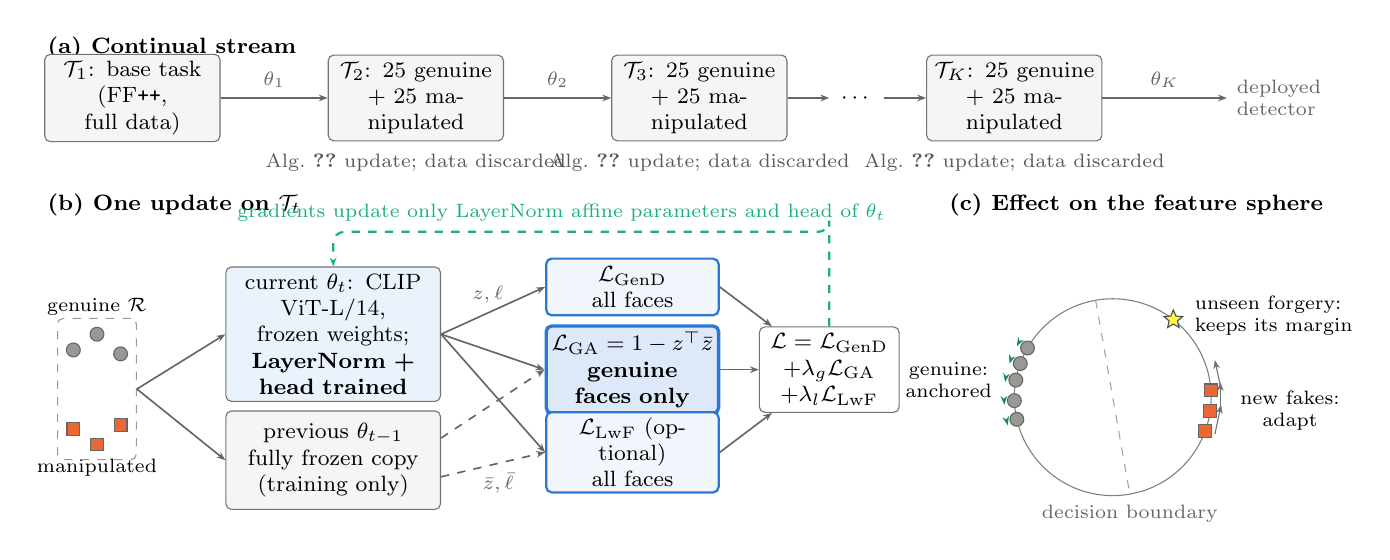
\begin{tikzpicture}[
  font=\footnotesize,
  >={Stealth[length=3.2pt]},
  box/.style={draw=black!55, rounded corners=2pt, align=center, inner sep=2.5pt},
  task/.style={box, fill=black!4, minimum height=0.85cm, text width=2.05cm},
  model/.style={box, minimum height=1.25cm, text width=2.55cm},
  loss/.style={draw=oursblue, thick, rounded corners=2pt, align=center, fill=oursblue!7, inner sep=2pt, minimum height=0.72cm, text width=2.05cm},
  gen/.style={circle, draw=black!60, fill=genc, inner sep=0pt, minimum size=5pt},
  fak/.style={rectangle, draw=black!60, fill=fakc, inner sep=0pt, minimum size=4.6pt},
  arr/.style={->, black!60, semithick},
  pan/.style={font=\footnotesize\bfseries, anchor=north west}]
% ---------------- (a) stream
\node[pan] at (-0.2,5.45) {(a) Continual stream};
\node[task] (t1) at (1.0,4.55) {$\mathcal{T}_1$: base task\\(\ffpp{}, full data)};
\node[task] (t2) at (4.6,4.55) {$\mathcal{T}_2$: 25 genuine\\+ 25 manipulated};
\node[task] (t3) at (8.2,4.55) {$\mathcal{T}_3$: 25 genuine\\+ 25 manipulated};
\node[task] (tk) at (12.2,4.55) {$\mathcal{T}_K$: 25 genuine\\+ 25 manipulated};
\node at (10.2,4.55) {$\cdots$};
\draw[arr] (t1) -- node[above, font=\scriptsize]{$\theta_1$} (t2);
\draw[arr] (t2) -- node[above, font=\scriptsize]{$\theta_2$} (t3);
\draw[arr] (t3) -- (9.85,4.55); \draw[arr] (10.55,4.55) -- (tk);
\draw[arr] (tk) -- node[above, font=\scriptsize]{$\theta_K$} (14.9,4.55) node[right, align=left, font=\scriptsize]{deployed\\detector};
\foreach \t in {t2,t3,tk} \node[font=\scriptsize, text=black!65, below=1pt of \t] {Alg.~\ref{alg:gad} update; data discarded};
% ---------------- (b) one update
\node[pan] at (-0.2,3.45) {(b) One update on $\mathcal{T}_t$};
\node[gen] (g1) at (0.25,1.35) {}; \node[gen] (g2) at (0.55,1.55) {}; \node[gen] (g3) at (0.85,1.3) {};
\node[fak] (f1) at (0.25,0.35) {}; \node[fak] (f2) at (0.55,0.15) {}; \node[fak] (f3) at (0.85,0.4) {};
\node[font=\scriptsize, align=center] at (0.55,1.9) {genuine $\mathcal{R}$};
\node[font=\scriptsize, align=center] at (0.55,-0.15) {manipulated};
\node[draw=black!40, dashed, rounded corners=2pt, fit=(g1)(g2)(g3)(f1)(f2)(f3), inner sep=3pt] (batch) {};
\node[model, fill=oursblue!10] (cur) at (3.55,1.55) {current $\theta_t$: CLIP\\ViT-L/14, frozen weights;\\\textbf{LayerNorm + head trained}};
\node[model, fill=black!4] (prev) at (3.55,-0.05) {previous $\theta_{t-1}$\\fully frozen copy\\(training only)};
\draw[arr] (batch.east) -- (cur.west);
\draw[arr] (batch.east) -- (prev.west);
\node[loss] (lgend) at (7.35,2.15) {$\mathcal{L}_{\mathrm{GenD}}$\\all faces};
\node[loss, very thick, fill=oursblue!16] (lga) at (7.35,1.1) {$\mathcal{L}_{\mathrm{GA}}=1-z^{\top}\bar z$\\\textbf{genuine faces only}};
\node[loss] (llwf) at (7.35,0.05) {$\mathcal{L}_{\mathrm{LwF}}$ (optional)\\all faces};
\draw[arr] (cur.east) -- node[above, font=\scriptsize, pos=0.45]{$z,\ell$} (lgend.west);
\draw[arr] (cur.east) -- (lga.west);
\draw[arr] (cur.east) -- (llwf.west);
\draw[arr, dashed] ([yshift=8pt]prev.east) -- (lga.west);
\draw[arr, dashed] ([yshift=-6pt]prev.east) -- node[below, font=\scriptsize, pos=0.55]{$\bar z,\bar\ell$} (llwf.west);
\node[box, fill=white, text width=1.6cm] (sum) at (9.85,1.1) {$\mathcal{L}=\mathcal{L}_{\mathrm{GenD}}$\\$+\lambda_g\mathcal{L}_{\mathrm{GA}}$\\$+\lambda_l\mathcal{L}_{\mathrm{LwF}}$};
\draw[arr] (lgend.east) -- (sum); \draw[arr] (lga.east) -- (sum); \draw[arr] (llwf.east) -- (sum);
\draw[->, thick, gradc, dashed, rounded corners=4pt] (sum.north) |- (9.85,2.85) -| node[pos=0.27, above, font=\scriptsize, text=gradc]{gradients update only LayerNorm affine parameters and head of $\theta_t$} (cur.north);
% ---------------- (c) hypersphere intuition
\node[pan] at (11.25,3.45) {(c) Effect on the feature sphere};
\def\R{1.25}
\coordinate (O) at (13.45,0.75);
\draw[black!50] (O) circle (\R);
\draw[black!35, dashed] ($(O)+(100:\R)$) -- ($(O)+(280:\R)$);
\node[font=\scriptsize, text=black!60, anchor=north] at ($(O)+(280:\R)+(0,-0.02)$) {decision boundary};
% genuine cluster: anchored (tiny moves)
\foreach \a in {150,160,170,182,193} {
  \node[gen] at ($(O)+(\a:\R)$) {};
  \draw[->, gradc!80!black, thin] ($(O)+(\a:\R)+(\a:0.13)$) -- ($(O)+(\a+2:\R)+(\a+2:0.13)$);
}
\node[font=\scriptsize, align=center, anchor=east] at ($(O)+(170:\R)+(-0.18,0)$) {genuine:\\anchored};
% stream fakes: free to move
\foreach \a in {-20,-8,4} {
  \node[fak] at ($(O)+(\a:\R)$) {};
  \draw[->, black!55, thin] ($(O)+(\a:\R)+(\a:0.13)$) -- ($(O)+(\a+16:\R)+(\a+16:0.13)$);
}
\node[font=\scriptsize, align=center, anchor=west] at ($(O)+(-8:\R)+(0.26,0)$) {new fakes:\\adapt};
% unseen fake keeps its margin
\node[star, star points=5, star point ratio=2.2, draw=black!70, fill=yellow!70, inner sep=0pt, minimum size=7pt] at ($(O)+(52:\R)$) {};
\node[font=\scriptsize, align=left, anchor=west] at ($(O)+(52:\R)+(0.15,0.05)$) {unseen forgery:\\keeps its margin};
\end{tikzpicture}

\caption{Training procedure studied in this paper. (a) The detector is trained once on the base task and then updated on a stream of few-shot tasks; each update uses only the current task's 25 genuine and 25 manipulated videos, which are discarded afterwards, so no exemplars or features are stored. (b) One update (Algorithm~\ref{alg:gad}): a frozen copy of the previous model supplies targets during training only; the GenD loss acts on all faces, the genuine-sample alignment $\mathcal{L}_{\mathrm{GA}}$ (the positive sample alignment of DFWF~\cite{ma2021dfwf}) acts on genuine faces only, and the logit distillation $\mathcal{L}_{\mathrm{LwF}}$ acts on all faces and is optional (Section~\ref{sec:matched}); gradients reach only the LayerNorm affine parameters and the head. (c) Schematic intuition, not data: genuine features stay anchored on the hypersphere while features of the new manipulations move, so forgeries that are never trained keep their margin to the genuine class (Section~\ref{sec:theory}).}
\label{fig:method}
\end{figure*}

\subsection{Ranking-margin analysis}
\label{sec:theory}
DFWF justified genuine alignment by the consistency of genuine samples. The following elementary argument relates it directly to the detection of forgeries that are never trained. Write the detector's decision score as the logit difference $s_\theta(x)=w^{\top}z_\theta(x)+c$, where $\|z_\theta(x)\|=1$, and let $\theta'$ denote the model after an update, with head $(w',c')$.

\begin{proposition}[Score shift]
\label{prop:shift}
For every input $x$, with angular drift $\delta(x)=1-z_{\theta'}(x)^{\top}z_\theta(x)$,
\begin{equation}
|s_{\theta'}(x)-s_\theta(x)|\le\|w'-w\|+|c'-c|+\|w\|\sqrt{2\,\delta(x)} .
\label{eq:shift}
\end{equation}
\end{proposition}
\begin{proof}
$s_{\theta'}(x)-s_\theta(x)=(w'-w)^{\top}z_{\theta'}(x)+w^{\top}\big(z_{\theta'}(x)-z_\theta(x)\big)+(c'-c)$. The first term is bounded by $\|w'-w\|$ because $\|z_{\theta'}(x)\|=1$, and $\|z_{\theta'}(x)-z_\theta(x)\|^2=2-2z_{\theta'}(x)^{\top}z_\theta(x)=2\delta(x)$.
\end{proof}

\begin{proposition}[Margin bound on unseen-manipulation AUROC]
\label{prop:auc}
Let $G$ be the distribution of genuine faces and $Q$ that of an unseen manipulation, and let $\mathrm{AUC}=P_{r\sim G,\,u\sim Q}\big(s_\theta(u)>s_\theta(r)\big)$. If $|s_{\theta'}(r)-s_\theta(r)|\le\epsilon_G$ for all genuine $r$ and $s_{\theta'}(u)\ge s_\theta(u)-\epsilon_Q$ for all $u$ from $Q$, then
\begin{equation}
\mathrm{AUC}-\mathrm{AUC}'\le P\big(0<s_\theta(u)-s_\theta(r)\le\epsilon_G+\epsilon_Q\big).
\label{eq:auc}
\end{equation}
\end{proposition}
\begin{proof}
If $s_\theta(u)-s_\theta(r)>\epsilon_G+\epsilon_Q$, then $s_{\theta'}(u)-s_{\theta'}(r)\ge s_\theta(u)-\epsilon_Q-s_\theta(r)-\epsilon_G>0$, so the pair stays correctly ranked. Only pairs whose margin before the update lies in $(0,\epsilon_G+\epsilon_Q]$ can become misranked.
\end{proof}

Proposition~\ref{prop:auc} states that an update can damage the detection of an unseen manipulation only through pairs with a small margin, and only by an amount governed by the score shift of genuine faces, $\epsilon_G$, and of the unseen manipulated faces, $\epsilon_Q$. During an update, $\epsilon_Q$ cannot be controlled directly, because no sample of $Q$ is available, and constraining the current manipulated faces does not target $Q$ while it opposes learning them. The genuine class is different: it occurs in every task, and the genuine faces of the current task are samples of the same class on which every future and unseen comparison relies. By Proposition~\ref{prop:shift}, the representation part of $\epsilon_G$ is controlled by the angular drift of genuine features, which is exactly the quantity that $\mathcal{L}_{\mathrm{GA}}$ penalizes, while the head terms of Proposition~\ref{prop:shift} are not controlled by GA. LwF encourages output consistency on the available update samples; it does not directly guarantee a uniform bound on classifier changes or on scores of unseen data. The argument is therefore a conditional motivation rather than a guarantee. The constraint acts on the genuine faces of the current task, and it protects genuine faces of other datasets only to the extent that it transfers to them. Section~\ref{sec:drift} tests this transfer: GA trained on stream data reduces the drift of genuine faces from WildDeepfake and DeepFakeFace, which no model ever saw.

Algorithm~\ref{alg:gad} gives the complete update.

\begin{algorithm}[t]
\caption{One GA+LwF update on task $\mathcal{T}_t$}
\label{alg:gad}
\footnotesize
\begin{algorithmic}[1]
\Require current parameters $\theta_{t-1}$ (LayerNorm affine and head), few-shot set $\mathcal{D}_t$, weights $\lambda_g,\lambda_l$, temperature $T$, epochs $E$
\State $\bar\theta\gets\theta_{t-1}$, frozen; $\theta_t\gets\theta_{t-1}$
\For{$e=1,\dots,E$}
  \For{each minibatch $\{(x_i,y_i)\}_{i\in\mathcal{B}}\subset\mathcal{D}_t$}
    \State $\tilde x_i\gets$ GenD augmentation of $x_i$
    \State $(\ell_i,z_i)\gets f_{\theta_t}(\tilde x_i)$; \ $(\bar\ell_i,\bar z_i)\gets f_{\bar\theta}(\tilde x_i)$ \Comment{same view}
    \State $\mathcal{R}\gets\{i\in\mathcal{B}:y_i=\text{genuine}\}$
    \State $\mathcal{L}\gets\mathcal{L}_{\mathrm{GenD}}+\lambda_l\,T^2\,\frac{1}{|\mathcal{B}|}\sum_{i\in\mathcal{B}}\mathrm{KL}\big(\sigma(\bar\ell_i/T)\,\|\,\sigma(\ell_i/T)\big)$
    \If{$\mathcal{R}\neq\emptyset$}
      \State $\mathcal{L}\gets\mathcal{L}+\lambda_g\frac{1}{|\mathcal{R}|}\sum_{i\in\mathcal{R}}\big(1-z_i^{\top}\bar z_i\big)$
    \EndIf
    \State update $\theta_t$ with Adam on $\nabla_{\theta_t}\mathcal{L}$
  \EndFor
\EndFor
\State discard $\bar\theta$; \Return $\theta_t$ \Comment{nothing is stored}
\end{algorithmic}
\end{algorithm}

Algorithm~\ref{alg:stream} gives the continual protocol in which the update is applied and evaluated, and Algorithm~\ref{alg:select} the development-data procedure we use to choose the alignment weight for a desired amount of plasticity (Section~\ref{sec:matched}).

\begin{algorithm}[t]
\caption{Continual updating and evaluation}
\label{alg:stream}
\footnotesize
\begin{algorithmic}[1]
\Require detector $\theta_1$ trained on base task $\mathcal{T}_1$, stream $\mathcal{T}_2,\dots,\mathcal{T}_K$, shots $n$, weights $\lambda_g,\lambda_l$
\For{$t=2,\dots,K$}
  \State $\mathcal{D}_t\gets n$ genuine and $n$ manipulated videos from the fitting pool of $\mathcal{T}_t$
  \State $\theta_t\gets$ \textsc{Update}$(\theta_{t-1},\mathcal{D}_t,\lambda_g,\lambda_l)$ \Comment{Algorithm~\ref{alg:gad}}
  \State discard $\mathcal{D}_t$ and $\theta_{t-1}$ \Comment{no exemplars or features kept}
  \For{$j=1,\dots,t$}
    \State $A_{t,j}\gets$ video AUROC of $\theta_t$ on the test split of $\mathcal{T}_j$
  \EndFor
\EndFor
\State $U\gets\frac12\big(\mathrm{AUC}_{\mathrm{WDF}}(\theta_K)+\frac13\sum_g\mathrm{AUC}_{\mathrm{DFF},g}(\theta_K)\big)$ \Comment{sealed panel}
\State compute AA, AF and gain from $\{A_{t,j}\}$
\State \Return $\theta_K$, AA, AF, gain, $U$
\end{algorithmic}
\end{algorithm}

\begin{algorithm}[t]
\caption{Development-selected alignment weight}
\label{alg:select}
\footnotesize
\begin{algorithmic}[1]
\Require candidate weights $\Lambda$, target plasticity $G^{*}$ (mean gain), development splits
\For{each $\lambda\in\Lambda$}
  \State run Algorithm~\ref{alg:stream} on the development splits with $\lambda_g=\lambda$
  \State $G(\lambda)\gets$ mean gain of the run
\EndFor
\State $\lambda^{*}\gets\arg\min_{\lambda\in\Lambda}|G(\lambda)-G^{*}|$ \Comment{ties: larger $\lambda$}
\State \Return $\lambda^{*}$ \Comment{sealed test data and panel never used}
\end{algorithmic}
\end{algorithm}


\section{Experimental Setup}
\label{sec:setup}

\subsection{Data and preprocessing}
Table~\ref{tab:data} lists the data. The base task is \ffpp{} c23 with its four manipulation methods, on which GenD is trained. The default stream S1 then adds DFDC-Preview~\cite{dolhansky2019dfdcpreview}, the DeepFakeDetection set (DFD) distributed with \ffpp{}~\cite{rossler2019faceforensics} and Celeb-DF~v2 (CDF)~\cite{li2020celebdf}, the order used by recent continual deepfake detection work~\cite{pan2023dfil,zhang2025gpl}. Two further orders follow the same work: S2 swaps the last two tasks (\ffpp{}, DFDC-P, CDF, DFD) and S3 learns DFD first (\ffpp{}, DFD, DFDC-P, CDF). Every split is identity disjoint. DFDC-P uses its official split after removing the two identities shared between train and test. DFD has no official split, and the widely used DeepfakeBench~\cite{yan2023deepfakebench} configuration places every DFD video in its training, validation and test sets simultaneously. We therefore divided its 28 actors into fitting, development and test groups and admitted a manipulated video involving actors $A$ and $B$ to a role only if both belong to it. For CDF, all 56 test identities also occur in non-test videos, so the fitting pool contains only identity-clean videos. In the first version of our splits, the CDF genuine samples were mostly YouTube videos while all CDF fakes derive from celebrity videos. Under this source confound, learning CDF reduced CDF accuracy. The corrected split draws genuine samples from celebrity videos only, and all reported results use it.

\begin{table}[t]
\caption{Datasets, roles and numbers of genuine/manipulated videos (images for DFF). Updates draw 25 genuine and 25 manipulated videos from the fitting pool.}
\label{tab:data}
\centering
\footnotesize
\setlength{\tabcolsep}{2.5pt}
\begin{tabular}{@{}llccc@{}}
\toprule
Dataset & Role & Fitting pool & Development & Test \\
\midrule
\ffpp{} c23~\cite{rossler2019faceforensics} & Base task & 720 / 2880 & 140 / 560 & 140 / 558 \\
DFDC-P~\cite{dolhansky2019dfdcpreview} & Update & 551 / 1599 & 262 / 272 & 230 / 424 \\
DFD~\cite{rossler2019faceforensics} & Update & 110 / 254 & 59 / 143 & 194 / 792 \\
Celeb-DF v2~\cite{li2020celebdf} & Update & 30 / 45 & 150 / 150 & 178 / 340 \\
FaceShifter~\cite{rossler2019faceforensics} & Dev.\ probe & \textendash & 140 / 140 & \textendash \\
WildDeepfake~\cite{zi2020wilddeepfake} & Sealed unseen & \textendash & \textendash & 396 / 410 \\
DeepFakeFace~\cite{song2023deepfakeface} & Sealed unseen & \textendash & \textendash & 1000 / 2967 \\
\bottomrule
\end{tabular}
\end{table}

Neither WildDeepfake nor DeepFakeFace was used by GenD for training or checkpoint selection, and both were registered and sealed before any model was evaluated on them. For WildDeepfake we use the official test split. For DeepFakeFace we use a fixed random sample of 1000 genuine images and 1000 images from each of its Stable Diffusion inpainting, InsightFace face-swap and Stable Diffusion text-to-image subsets, of which 998, 1000 and 969 contained a detectable face.

\textit{Preprocessing.} Video datasets are processed with the GenD face pipeline at 32 frames per video. Manipulated videos of \ffpp{} and DFD are cropped with the official manipulation masks, which select the manipulated face in multi-person scenes. Without masks, the largest-face rule crops bystanders in DFD scenes such as group meetings and reduces GenD's DFD AUROC from 97.59 to 91.40. The DFD masks are distributed as fragmented MP4 files whose frame count is not readable by the standard decoder, and we remuxed them losslessly. Because masks exist only for manipulated videos, face selection depends on the label for these two datasets; Section~\ref{sec:labelindep} repeats the evaluation with label-independent largest-face crops. The unseen panel involves no masks. DFDC-P and WildDeepfake are distributed as face crops, which we re-detected and re-aligned with the same pipeline. Because WildDeepfake crops are tight, a 25\% border was added before detection, which raised the detection rate from 30\% to 99.8\% of frames; this change was fixed before the panel was scored.

\subsection{Compared methods}
All methods start from the same detector and train the same parameters with $\mathcal{L}_{\mathrm{GenD}}$ unless stated otherwise. Sequential fine-tuning (Seq.\ FT) uses no regularizer, and head-only fine-tuning freezes the LayerNorm parameters and trains the 2{,}050 head parameters. EWC~\cite{kirkpatrick2017ewc} adds a diagonal Fisher penalty, LayerNorm merging averages the trainable parameters across tasks, and LwF~\cite{li2018lwf} adds logit distillation. Symmetric KD applies the feature distillation term to all faces, and its combination with LwF corresponds to the all-sample representation and output distillation used by CoReD-style methods~\cite{kim2021cored}. Two mechanism controls change only the samples on which features are distilled: fake-only KD distills manipulated faces, and random-subset KD distills a random subset of each batch that contains as many samples as the batch has genuine faces. Exemplar replay keeps five genuine and five manipulated raw videos from every earlier task and mixes them into training; it violates the exemplar-free constraint and serves as a reference. Joint training learns once from the union of all few-shot sets, including a few-shot sample of \ffpp{}. During development we also evaluated prototype replay with semantic drift compensation and GA combined with this prototype memory.

GPL~\cite{zhang2025gpl} has no public code, so we re-implemented it from the paper and its supplement on the same detector and protocol. As in GPL, the detector is frozen during updates (here the LayerNorm parameters and head of GenD), and only a lightweight watermark generator is trained: three convolutional layers produce a sample-specific mask that modulates a learned watermark added to the input (156{,}659 parameters). The loss combines cross-entropy with GPL's hyperbolic contrastive alignment to 25 genuine and 25 manipulated cluster centers of the base task ($\lambda_{\mathrm{nce}}=0.1$, GPL's best value), and the task gradient is projected against the gradient of the divergence from the previous model whenever the two conflict. Settings that GPL does not report (zero-initialized watermark, temperature 0.1, full removal of the conflicting gradient component, exponential map of unit-norm features into the Poincar\'e ball) were fixed before any run. Because the watermark generator is a newly initialized module, its learning rate was selected on development data with a registered rule, as the configuration of GA was: $10^{-4}$ barely learned (mean gain 0.01) and $10^{-3}$ was chosen. GPL stores the base-task cluster centers, a small set of feature statistics, but no images.

\subsection{Protocol, statistics and implementation}
The study has three stages. Development used the released GenD checkpoint, development splits and three seeds, and it selected the configuration that was then confirmed. Confirmation used a GenD model that we retrained on \ffpp{} following the authors' recipe but selected on \ffpp{} validation data only (epoch 8), together with the sealed test splits and the sealed unseen panel. The released checkpoint was selected on a validation pool that includes Celeb-DF-family data, so its cross-dataset scores are not strictly zero-shot. The extension stage added 43 runs from the same retrained model with one training seed. A second extension, registered after an external review, added the GPL comparison, four more training seeds for the main methods and a nine-update stream (42 runs), and a third added matched-plasticity runs and the analyses requested by a second review. Every stage was registered before its runs: hypotheses, primary score, decision rules and amendments were written down and hashed, and no method, hyperparameter or preprocessing choice was made from confirmation or extension results. The registrations were stored locally with their hashes and file dates and were not deposited with an independent timestamping service, so their dates cannot be verified independently; the code, split manifests, registrations and result summaries are available at \url{https://github.com/NarenTheNumpkin/Protecting-Generalization-in-Continually-Updated-Deepfake-Detectors}. The extensions re-use the sealed data scored in the confirmation stage.

A hypothesis is confirmed if the difference in $U$ is positive and its paired 95\% bootstrap interval excludes zero. We use 2000 resamples; WildDeepfake is resampled by source video within each class, and DeepFakeFace by image, with the genuine images resampled once and shared by the three generator comparisons, as they are in the score itself. The registered hypotheses form families that are tested separately: confirmation (3), mechanism controls (3), replication (12), robustness (3), comparison with GPL (4), five seeds (5), the nine-update stream (3) and matched plasticity (2). Over the first three families together we additionally control the family-wise error rate with the Holm procedure~\cite{holm1979}, using one-sided bootstrap $p$-values from 10{,}000 resamples, and the seed and matched-plasticity families are Holm-corrected within themselves. Differences in AA on the test splits are given with paired bootstrap intervals that resample identity clusters within each class and dataset. A difference that is not significant does not show equivalence; where we state that a score is retained, we give the interval of the difference to the never-updated detector and, as an exploratory post hoc analysis, compare it with a margin of one AUROC point (Section~\ref{sec:retention}). These intervals reflect test-sample variability but not variability across training runs. For the main comparison on stream S1 we therefore also train with five seeds, which change the few-shot samples and all training randomness while keeping the initial GenD model fixed, and test differences in $U$ with one-sided paired $t$-tests across seeds, Holm-corrected over the five registered comparisons. The other settings use one seed and rely on replication across task orders, backbones, regularization strengths and data regimes.

\textit{Implementation.} Trainable parameters start from the GenD checkpoint (the GPL watermark from zero, its convolutions from the PyTorch default initialization). Inputs are face crops resized and center-cropped to $224\times224$ and normalized with the CLIP mean and standard deviation. Every method uses ten epochs per task over all 32 frames of the 50 few-shot videos, shuffled each epoch without class stratification, Adam ($\beta=(0.9,0.999)$, no weight decay) with learning rate $10^{-4}$ and cosine decay to zero without warm-up, batch size 16, bfloat16 precision and GenD's default training augmentations; there is no early stopping, and the model after the last epoch is kept. Settings were fixed before the experiments from the GenD defaults, with $\lambda=1$ for every regularizer; no method was tuned individually, except the learning rate of the GPL watermark generator (Section~\ref{sec:setup}) and the development-selected settings of Section~\ref{sec:matched}. Unless stated otherwise, test splits are scored with eight evenly spaced frames per video; the calibration, per-manipulation and operating-point analyses use all 32 frames. Video scores are the mean frame probability. All experiments run on a single NVIDIA RTX 5060 Ti (16~GB) with Python 3.12, PyTorch 2.8.0 (CUDA 12.8) and Transformers 4.56.2; seeds fix the few-shot samples and all training randomness.

\section{Results}
\label{sec:results}

\subsection{Reproduction and the cost of updates}
Table~\ref{tab:repro} compares reported and reproduced GenD scores. With the released weights, our pipeline reproduces the reported Celeb-DF and DFD results. The retrained model with clean checkpoint selection is equally strong in domain, but it is 3.1 points lower on Celeb-DF (2.6 points below the reported value) and 4.3 points lower on DFDC-P than the released weights. Part of the published cross-dataset performance therefore appears to depend on checkpoint selection. The accuracy reported by the official evaluation code uses the equal-error threshold computed on the test labels, so we report accuracy at a fixed threshold throughout.

\begin{table}[t]
\caption{Video AUROC (\%) of GenD. Released weights are evaluated with our pipeline; the retrained model selects its checkpoint on \ffpp{} validation only. Dashes denote values that were not reported or not evaluated.}
\label{tab:repro}
\centering
\footnotesize
\setlength{\tabcolsep}{4pt}
\begin{tabular}{@{}lccc@{}}
\toprule
Test set & Paper~\cite{yermakov2026gend} & Released weights & Clean retrain \\
\midrule
\ffpp{} test & \textendash & \textendash & 98.21 \\
Celeb-DF v2 & 94.6 & 95.11 [92.95, 96.81] & 92.04 \\
DFD & 96.4 & 97.59 [96.80, 98.30] & \textendash \\
DFDC-P & \textendash & 90.00 & 85.66 \\
\bottomrule
\end{tabular}
\end{table}

\textit{Cost of an update.} Starting from the released checkpoint, sequential fine-tuning on stream S1 learns every task (mean gain 2.10 AUROC points) and forgets little (average forgetting 0.79 points). Two costs, however, are large and consistent across seeds. Detection of the never-trained FaceShifter manipulation falls from 84.85 to 77.06 AUROC (range over seeds 76.44 to 77.39). The accuracy of the base task at a fixed threshold drops from 95.0\% to 79.9\%, although its AUROC remains above 95. Updating a generalizable detector therefore mainly damages its generalization and its calibration.

\begin{table}[t]
\caption{Development results (released GenD, development splits with 8 frames per video, three seeds). FSh: FaceShifter probe AUROC after all updates, mean and [min, max] over seeds.}
\label{tab:dev}
\centering
\footnotesize
\setlength{\tabcolsep}{2.6pt}
\begin{tabular}{@{}lcccccc@{}}
\toprule
Method & FSh & AA & AF & Gain & ACC$_{\mathrm{FF}}$ \\
\midrule
No update & 84.85 & 97.20 & \textendash & \textendash & 95.0 \\
Seq.\ FT & 77.06 [76.44, 77.39] & 97.78 & 0.79 & 2.10 & 79.9 \\
EWC~\cite{kirkpatrick2017ewc} & 76.67 [75.52, 77.34] & 97.73 & 0.84 & 2.10 & 79.7 \\
SDC replay & 76.94 [75.66, 78.65] & 97.70 & 0.86 & 2.05 & 78.9 \\
Symmetric KD & 78.66 [77.57, 79.48] & 98.18 & 0.31 & 1.51 & 85.1 \\
LN merging & 80.38 [79.94, 81.01] & 97.57 & 0.30 & 0.85 & 88.1 \\
LwF~\cite{li2018lwf} & 80.49 [80.23, 80.69] & 97.95 & 0.30 & 1.39 & 86.3 \\
GA + memory & 80.69 [79.54, 81.58] & 98.42 & 0.13 & 1.38 & 87.6 \\
GA & 80.67 [79.30, 81.63] & 98.42 & 0.13 & 1.40 & 87.8 \\
GA + mem.\ + LwF & 82.84 [81.99, 83.38] & 98.26 & $-$0.01 & 1.05 & 91.1 \\
GA+LwF & \textbf{82.85} [82.05, 83.52] & 98.26 & 0.01 & 1.05 & \textbf{91.5} \\
\bottomrule
\end{tabular}
\end{table}

\begin{figure}[t]
\centering
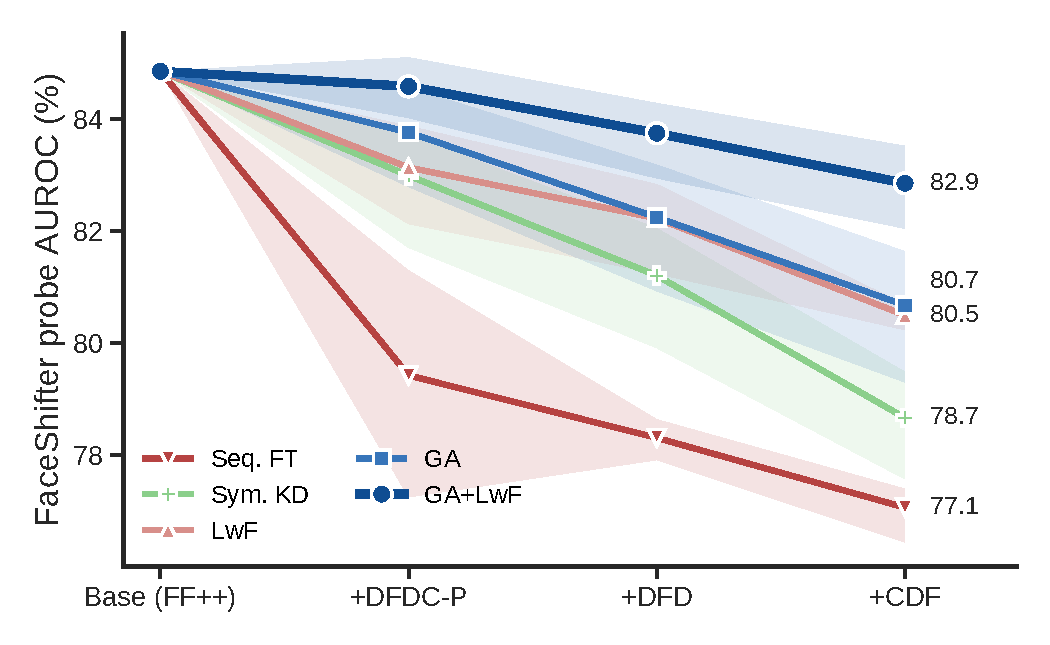
\includegraphics[width=\columnwidth]{figures/fig_dev_curves.pdf}
\caption{FaceShifter probe AUROC across the update stream on development data. Lines show the mean and shaded bands the range over three seeds.}
\label{fig:dev}
\end{figure}

\textit{Development comparison.} Table~\ref{tab:dev} and Fig.~\ref{fig:dev} report the development results over three seeds. Restricting feature distillation to genuine faces improves the FaceShifter probe over symmetric distillation in all six paired comparisons, by 2.0 points on average, with higher AA and lower forgetting. A prototype memory added to GA changed nothing and was removed. GA and LwF were complementary in development (82.85, about two points above either component), at a cost in plasticity (gain 1.05 against 2.10 for sequential fine-tuning).

\begin{table*}[t]
\caption{Stream S1 from the clean retrained GenD (seed 0). Unseen panel AUROC (all frames) and sealed test-split video AUROC (8 frames per video) after all updates. $U$: unseen-panel score; AF: average forgetting (negative values indicate backward transfer); ACC$_{\mathrm{FF}}$: base-task accuracy at threshold 0.5. Replay stores raw videos and joint training learns all tasks at once; both are references, not exemplar-free continual methods. $^\dagger$Our re-implementation on GenD; it stores base-task feature cluster centers.}
\label{tab:main}
\centering
\footnotesize
\setlength{\tabcolsep}{4pt}
\begin{tabular}{@{}lc|cccc|cccc|cccc@{}}
\toprule
& & \multicolumn{4}{c|}{Unseen panel} & \multicolumn{4}{c|}{Trained datasets (test)} & & & & \\
Method & Stores data & $U$ & WDF & DFF & DFF-T2I & \ffpp{} & DFDC-P & DFD & CDF & AA & AF & Gain & ACC$_{\mathrm{FF}}$ \\
\midrule
No update & no & 87.97 & 90.91 & 85.03 & 78.02 & 98.06 & 85.71 & 97.38 & 91.92 & 93.27 & \textendash & \textendash & 94.1 \\
Head-only FT & no & 88.11 & 91.27 & 84.94 & 77.97 & 98.05 & 85.34 & 97.70 & 92.19 & 93.32 & 0.05 & 0.02 & 94.3 \\
Seq.\ FT & no & 86.17 & 91.80 & 80.55 & 65.16 & 96.69 & 90.83 & 96.64 & 94.88 & 94.76 & $-$1.24 & 0.83 & 84.7 \\
EWC~\cite{kirkpatrick2017ewc} & no & 86.28 & 91.63 & 80.94 & 65.90 & 96.62 & 90.79 & 96.83 & 94.86 & 94.77 & $-$1.30 & 0.95 & 84.2 \\
Fake-only KD & no & 86.47 & 91.95 & 80.99 & 67.10 & 97.65 & 88.78 & 96.29 & 94.55 & 94.32 & $-$0.64 & 0.58 & 88.5 \\
LwF~\cite{li2018lwf} & no & 86.88 & 91.86 & 81.91 & 68.99 & 97.98 & 89.56 & 97.18 & 94.47 & 94.80 & $-$0.98 & 0.92 & 90.4 \\
Random-subset KD & no & 86.94 & 92.20 & 81.69 & 68.19 & 97.82 & 88.90 & 97.06 & 95.22 & 94.75 & $-$0.94 & 0.68 & 90.0 \\
Symmetric KD & no & 86.95 & 92.16 & 81.75 & 68.36 & 97.83 & 88.99 & 97.09 & 95.24 & 94.79 & $-$0.96 & 0.69 & 89.8 \\
LN merging & no & 87.53 & 91.59 & 83.47 & 73.17 & 97.89 & 87.18 & 97.47 & 93.26 & 93.95 & $-$0.41 & 0.37 & 90.7 \\
Symmetric KD + LwF & no & 87.54 & 91.83 & 83.25 & 72.52 & 98.26 & 87.89 & 97.69 & 94.41 & 94.56 & $-$0.69 & 0.67 & 92.3 \\
GPL~\cite{zhang2025gpl}$^\dagger$ & centers & 85.74 & 90.89 & 80.59 & 71.50 & 95.99 & 92.28 & 95.26 & 95.59 & 94.78 & 0.69 & 2.51 & 87.0 \\
GA & no & 87.45 & 92.42 & 82.48 & 69.77 & 98.09 & 89.40 & 97.99 & 95.44 & \textbf{95.23} & $-$1.34 & 0.75 & 91.5 \\
GA+LwF & no & \textbf{87.88} & 91.91 & \textbf{83.86} & \textbf{73.77} & \textbf{98.32} & 88.23 & \textbf{98.15} & 94.41 & 94.78 & $-$0.85 & 0.74 & \textbf{93.7} \\
\midrule
Replay (5+5 videos/task) & yes & 86.34 & 91.81 & 80.86 & 66.96 & 96.80 & 90.18 & 96.97 & 95.18 & 94.78 & $-$1.30 & 1.01 & 87.7 \\
Joint training & yes & 87.48 & 92.33 & 82.64 & 70.40 & 97.21 & 87.61 & 98.05 & 94.87 & 94.43 & \textendash & \textendash & 89.8 \\
\bottomrule
\end{tabular}
\end{table*}

\begin{table}[t]
\caption{Pre-registered hypotheses on the unseen-panel score $U$. A hypothesis is confirmed if $\Delta U>0$ and its paired bootstrap 95\% interval excludes zero. $p_{\mathrm{H}}$: Holm-adjusted one-sided $p$-value over all 18 tests (10{,}000 resamples; the smallest attainable value is 0.0018). C1: confirmation stage; M: mechanism controls; R: replication.}
\label{tab:hyp}
\centering
\footnotesize
\setlength{\tabcolsep}{2.4pt}
\begin{tabular}{@{}llccc@{}}
\toprule
Hypothesis & Setting & $\Delta U$ & 95\% CI & $p_{\mathrm{H}}$ \\
\midrule
C1 GA+LwF $>$ LwF & S1 & +1.00 & [+0.70, +1.28] & 0.002 \\
C1 GA+LwF $>$ Seq.\ FT & S1 & +1.71 & [+1.01, +2.42] & 0.002 \\
C1 GA $>$ Sym.\ KD & S1 & +0.49 & [+0.31, +0.69] & 0.014 \\
\midrule
M1 GA $>$ random-subset KD & S1 & +0.51 & [+0.33, +0.70] & 0.002 \\
M2 GA $>$ fake-only KD & S1 & +0.98 & [+0.66, +1.35] & 0.002 \\
M3 GA+LwF $>$ Sym.\ KD+LwF & S1 & +0.34 & [+0.23, +0.47] & 0.002 \\
\midrule
R1 GA+LwF $>$ LwF & S2 & +0.80 & [+0.47, +1.15] & 0.002 \\
 & S3 & +1.14 & [+0.84, +1.49] & 0.002 \\
 & PE & +2.39 & [+1.57, +3.32] & 0.002 \\
R2 GA+LwF $>$ Seq.\ FT & S2 & +0.69 & [+0.06, +1.35] & 0.014 \\
 & S3 & +1.82 & [+1.13, +2.48] & 0.002 \\
 & PE & +2.13 & [+1.07, +3.20] & 0.002 \\
R3 GA $>$ Sym.\ KD & S2 & +0.37 & [+0.18, +0.56] & 0.002 \\
 & S3 & +0.54 & [+0.33, +0.76] & 0.002 \\
 & PE & +0.78 & [+0.44, +1.12] & 0.002 \\
R4 GA+LwF $>$ Sym.\ KD+LwF & S2 & +0.34 & [+0.23, +0.47] & 0.002 \\
 & S3 & +0.44 & [+0.31, +0.59] & 0.002 \\
 & PE & +0.58 & [+0.30, +0.87] & 0.002 \\
\bottomrule
\end{tabular}
\end{table}

\subsection{Main comparison on sealed data}
Table~\ref{tab:main} reports all methods on stream S1, starting from the clean retrained model and evaluated on the sealed test splits and the sealed unseen panel. GA+LwF keeps the unseen score close to that of the never-updated detector ($U=87.88$ against 87.97; Section~\ref{sec:retention} gives intervals and the loss per forgery family), whereas LwF loses 1.09 points and sequential fine-tuning 1.80 points. The three confirmatory hypotheses of this stage hold (Table~\ref{tab:hyp}). GA+LwF exceeds LwF by 1.00 points and sequential fine-tuning by 1.71 points, and GA exceeds symmetric distillation by 0.49 points. The registered guardrails also hold in this run: the AA of GA+LwF is within 0.5 points of the best method, and its mean gain is at least half that of sequential fine-tuning. Over five seeds the second guardrail is narrowly missed, at 47\% (Section~\ref{sec:seeds}).

The updates remain useful. Relative to the never-updated model, GA+LwF raises DFDC-P from 85.71 to 88.23, Celeb-DF from 91.92 to 94.41 and DFD from 97.38 to 98.15. It slightly improves the base task while keeping its fixed-threshold accuracy at 93.7\%, compared with 84.7\% after sequential fine-tuning. Fig.~\ref{fig:tradeoff} places every method in the plane of learning and generalization. Head-only fine-tuning attains the highest $U$ (88.11) only because it barely learns: its gain is 0.02 points and its AA essentially equals that of the never-updated model (93.32 against 93.27). GA and GA+LwF lie on the upper frontier among methods that learn the new datasets. GA favors the trained datasets (the highest AA, 95.23), and GA+LwF favors the unseen ones. Neither exemplar replay nor joint training on the union of the few-shot sets is an upper bound for retention: both store data yet reach a lower $U$ than GA+LwF. On the trained datasets, no statistically significant difference from the main competitors was detected, which does not establish equivalence. With 32-frame predictions and intervals that resample identity clusters, the AA of GA+LwF does not differ significantly from that of sequential fine-tuning ($-0.22$, 95\% interval $[-0.83,+0.42]$), EWC, replay, LwF ($-0.12$, $[-0.43,+0.17]$), symmetric KD ($-0.19$, $[-0.57,+0.21]$) or GPL ($-0.24$, $[-0.98,+0.52]$). It is higher than that of the never-updated model ($+1.52$, $[+1.07,+2.01]$) and of symmetric KD+LwF ($+0.14$, $[+0.01,+0.27]$), and lower than that of GA alone ($-0.59$, $[-0.90,-0.29]$).

\begin{figure}[t]
\centering
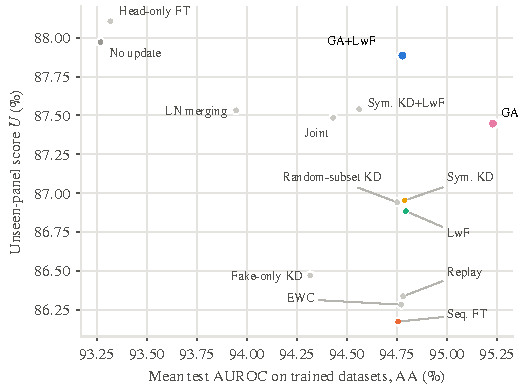
\includegraphics[width=\columnwidth]{figures/fig_tradeoff_all.pdf}
\caption{Learning versus generalization for all methods on stream S1 (sealed data). Methods in the upper left preserve generalization by learning little; GA and GA+LwF lie on the upper frontier among methods that learn.}
\label{fig:tradeoff}
\end{figure}

\begin{figure}[t]
\centering
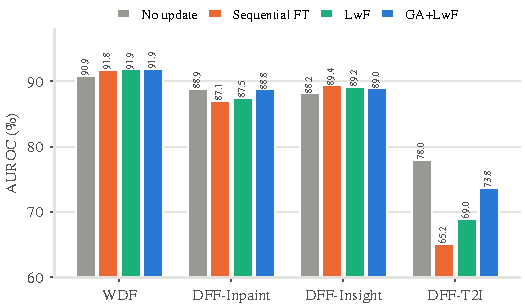
\includegraphics[width=\columnwidth]{figures/fig_unseen_breakdown.pdf}
\caption{Sealed unseen datasets after all updates on stream S1. Most of the generalization lost by updating concerns fully synthetic faces (DFF text-to-image), where GA+LwF retains 73.8 AUROC against 65.2 for sequential fine-tuning.}
\label{fig:unseen}
\end{figure}

Fig.~\ref{fig:unseen} shows where generalization is lost. On real-world WildDeepfake videos every update slightly improves detection, from 90.91 to between 91.27 and 92.42, presumably because the stream adds diverse face-swap examples. The loss is concentrated on DeepFakeFace, and above all on fully synthetic text-to-image faces, where sequential fine-tuning falls from 78.02 to 65.16 and GA+LwF retains 73.77. Updates on face-swap data thus erode sensitivity to generation families that are absent from the stream, and anchoring the genuine representation limits this erosion most.

\textit{Retention by forgery family.}\label{sec:retention} The unseen score averages forgery families that behave differently, and a difference that is not significant does not by itself show that performance is retained. Table~\ref{tab:retention} therefore reports the change relative to the never-updated detector for each family over the five training seeds, with 95\% intervals from a two-level bootstrap over seeds and test units. For GA+LwF the aggregate change is $-0.19$ points, with a 95\% interval of $[-0.62,+0.30]$; seed 0 alone gives $-0.09$ ($[-0.53,+0.43]$). The interval excludes losses larger than 0.62 points but does not exclude a small loss. In an exploratory analysis with a margin of one AUROC point, which we chose after the point estimates were known and which therefore does not constitute prospective confirmation, the lower bound lies above $-1$. Among the alternatives in Table~\ref{tab:retention}, the intervals of LwF, GPL and sequential fine-tuning lie entirely below zero; the development-selected GA-only setting of Section~\ref{sec:matched} was not part of this analysis. The aggregate hides opposite movements. WildDeepfake improves under GA+LwF ($+1.09$), as does the InsightFace face swap ($+0.56$), whereas text-to-image faces lose 4.66 points ($[-5.68,-3.70]$). Text-to-image faces are the worst family for every method, so retention is incomplete for fully synthetic faces, although GA+LwF loses less there than GPL ($-6.82$), LwF ($-8.92$) and sequential fine-tuning ($-14.83$).

\begin{table}[t]
\caption{Change of unseen-panel AUROC relative to the never-updated detector after all S1 updates, mean over five seeds, with 95\% intervals (one decimal) from a two-level bootstrap over seeds and test units. Inpaint., Swap, T2I: DeepFakeFace generators.}
\label{tab:retention}
\centering
\footnotesize
\setlength{\tabcolsep}{0.9pt}
\begin{tabular}{@{}lccccc@{}}
\toprule
Method & $U$ & WDF & Inpaint. & Swap & T2I \\
\midrule
GA+LwF & $-$0.19 & $+$1.09 & $-$0.30 & $+$0.56 & $-$4.66 \\
 & {\scriptsize[$-$0.6,\,0.3]} & {\scriptsize[0.3,\,2.0]} & {\scriptsize[$-$0.8,\,0.2]} & {\scriptsize[0.2,\,0.9]} & {\scriptsize[$-$5.7,\,$-$3.7]} \\[1pt]
LwF & $-$1.18 & $+$1.02 & $-$1.62 & $+$0.42 & $-$8.92 \\
 & {\scriptsize[$-$1.7,\,$-$0.6]} & {\scriptsize[0.1,\,2.1]} & {\scriptsize[$-$2.5,\,$-$0.8]} & {\scriptsize[$-$0.2,\,1.0]} & {\scriptsize[$-$10.2,\,$-$7.7]} \\[1pt]
GPL$^\dagger$ & $-$2.65 & $-$1.13 & $-$4.31 & $-$1.38 & $-$6.82 \\
 & {\scriptsize[$-$3.9,\,$-$1.4]} & {\scriptsize[$-$3.4,\,1.1]} & {\scriptsize[$-$5.6,\,$-$3.1]} & {\scriptsize[$-$2.3,\,$-$0.4]} & {\scriptsize[$-$9.1,\,$-$5.0]} \\[1pt]
Seq.\ FT & $-$2.77 & $+$0.72 & $-$3.91 & $-$0.03 & $-$14.83 \\
 & {\scriptsize[$-$3.8,\,$-$1.6]} & {\scriptsize[$-$0.9,\,2.6]} & {\scriptsize[$-$5.7,\,$-$2.3]} & {\scriptsize[$-$1.1,\,1.0]} & {\scriptsize[$-$16.9,\,$-$12.8]} \\[1pt]
\bottomrule
\end{tabular}
\end{table}

\begin{table}[t]
\caption{Per-manipulation test AUROC after all updates on stream S1 (32 frames per video). Each column compares the genuine test videos of the dataset with one manipulation method. FSh: FaceShifter probe (\ffpp{} development identities, never trained; 8 frames per video).}
\label{tab:permanip}
\centering
\footnotesize
\setlength{\tabcolsep}{2.7pt}
\begin{tabular}{@{}lccccccc@{}}
\toprule
& \multicolumn{4}{c}{\ffpp{} (base task)} & \multicolumn{2}{c}{DFDC-P} & \\
\cmidrule(lr){2-5}\cmidrule(lr){6-7}
Method & DF & F2F & FS & NT & A & B & FSh \\
\midrule
No update & 99.41 & 98.54 & 98.91 & 95.98 & 85.66 & 85.70 & 83.70 \\
Head-only FT & 99.37 & 98.55 & 98.97 & 95.83 & 85.20 & 85.75 & 83.67 \\
Seq.\ FT & 99.55 & 98.53 & 99.76 & 90.79 & 90.92 & 92.01 & 78.34 \\
EWC & 99.54 & 98.45 & 99.73 & 90.59 & 90.70 & 93.12 & 77.63 \\
Replay & 99.51 & 98.42 & 99.77 & 91.08 & 89.65 & 93.83 & 79.76 \\
LwF & 99.54 & 98.90 & 99.50 & 95.03 & 89.61 & 88.81 & 80.93 \\
Symmetric KD & 99.49 & 98.94 & 99.55 & 94.64 & 89.14 & 88.13 & 80.31 \\
Sym.\ KD + LwF & 99.48 & 98.86 & 99.34 & 95.82 & 88.04 & 87.12 & 82.72 \\
GA & 99.48 & 98.87 & 99.58 & 95.27 & 89.54 & 88.31 & 81.80 \\
GA+LwF & 99.47 & 98.86 & 99.41 & 95.88 & 88.19 & 87.29 & 83.19 \\
\bottomrule
\end{tabular}
\end{table}

\textit{Per-manipulation results.} Table~\ref{tab:permanip} breaks the trained datasets down by manipulation method, using 32-frame predictions, and adds the FaceShifter probe, which belongs to \ffpp{} but was never trained. On the base task, forgetting is concentrated on a single method. NeuralTextures, the most subtle \ffpp{} manipulation, falls from 95.98 to 90.79 under sequential fine-tuning and to 90.59 under EWC, while the other three methods stay above 98.4 for every model. GA+LwF keeps NeuralTextures at 95.88, the highest value among the methods that learn. On DFDC-P, the methods that learn most aggressively gain most, up to 93.83 on method B for replay against 87.29 for GA+LwF. This is the plasticity price discussed in Section~\ref{sec:discussion}. FaceShifter, starting from the clean retrained model, shows the same pattern as in development: sequential fine-tuning loses 5.4 points (83.70 to 78.34) and GA+LwF loses only 0.5 (83.19), less than any other method that learns.

\begin{table}[t]
\caption{Test AUROC (8 frames per video) of the final S1 models with mask-based crops of manipulated videos (mask) and with largest-face crops for every video (largest). AA: mean over the four trained datasets (DFDC-P and Celeb-DF involve no masks).}
\label{tab:labelindep}
\centering
\footnotesize
\setlength{\tabcolsep}{2.6pt}
\begin{tabular}{@{}lcccccc@{}}
\toprule
& \multicolumn{2}{c}{\ffpp{}} & \multicolumn{2}{c}{DFD} & \multicolumn{2}{c}{AA} \\
\cmidrule(lr){2-3}\cmidrule(lr){4-5}\cmidrule(lr){6-7}
Method & mask & largest & mask & largest & mask & largest \\
\midrule
No update & 98.06 & 97.85 & 97.38 & 90.82 & 93.27 & 91.58 \\
Seq.\ FT & 96.69 & 96.56 & 96.64 & 91.60 & 94.76 & 93.47 \\
LwF & 97.98 & 97.76 & 97.18 & 92.03 & 94.80 & 93.46 \\
Sym.\ KD+LwF & 98.26 & 98.11 & 97.69 & 92.50 & 94.56 & 93.23 \\
GPL$^\dagger$ & 95.99 & 95.78 & 95.26 & 90.72 & 94.78 & 93.59 \\
GA & 98.09 & 97.95 & 97.99 & 92.66 & 95.23 & 93.86 \\
GA+LwF & 98.32 & 98.15 & 98.15 & 92.50 & 94.78 & 93.32 \\
\bottomrule
\end{tabular}
\end{table}

\textit{Label-independent face selection.}\label{sec:labelindep} Masks exist only for manipulated videos, so the \ffpp{} and DFD test crops used so far depend on the label. We re-scored every final model with largest-face crops for all videos (Table~\ref{tab:labelindep}). \ffpp{} changes by at most 0.21 points, because its videos rarely contain more than one face. DFD AUROC, however, falls by 4.5 to 6.6 points for every model, including the never-updated detector (97.38 to 90.82): in multi-person DFD scenes the largest face is often a genuine bystander, so part of the manipulated videos is represented by genuine faces. Mask-based numbers therefore overstate the DFD performance attainable without knowing which face is manipulated. The comparison between updating methods changes little. Under the label-independent protocol the methods that learn lie within 0.7 AA points of each other (93.23 to 93.86) and 1.6 to 2.3 points above the never-updated detector, GA+LwF reaches 93.32 against 93.47 for sequential fine-tuning, and the rank correlation of the methods' AA between the two protocols is 0.60 (Kendall's $\tau$). The unseen panel, on which all retention results rest, involves no masks.

\textit{Mechanism controls.} Distilling only genuine faces constrains fewer samples than distilling all faces, so a weaker constraint, rather than the choice of the genuine class, could explain the advantage. Random-subset KD distills exactly as many samples per batch as GA, but chosen regardless of label. It reaches $U=86.94$, indistinguishable from symmetric KD (86.95), and GA exceeds it by 0.51 points (M1). Fake-only KD, the mirror image of GA, is the worst distillation variant ($U=86.47$, M2: GA better by 0.98 points); its AA is also lower (94.32). Within the combined method, replacing genuine-only feature distillation by symmetric feature distillation lowers $U$ by 0.34 points (M3). The effect is therefore tied to the genuine class and not to the number of distilled samples.

\begin{figure*}[t]
\centering
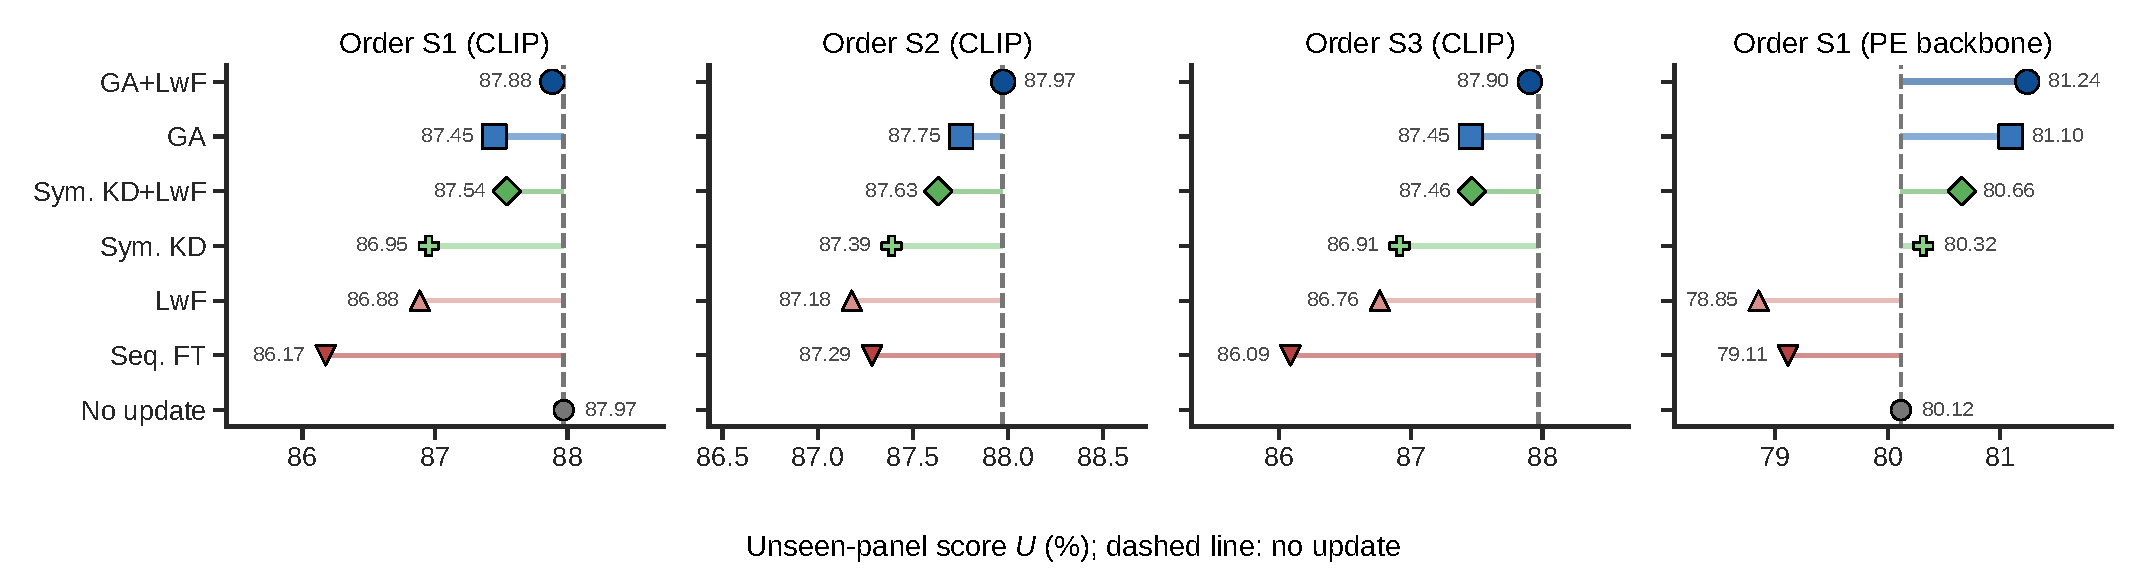
\includegraphics[width=\textwidth]{figures/fig_replication.pdf}
\caption{Unseen-panel score after all updates for the main methods in four settings: three task orders with the clean retrained CLIP-based GenD and order S1 with the released Perception Encoder variant. The dashed line marks the never-updated detector of each setting.}
\label{fig:replication}
\end{figure*}

\subsection{Generality of the result}
\textit{Task orders and backbones.} Fig.~\ref{fig:replication} repeats the comparison for orders S2 and S3 and for the Perception Encoder (PE) variant of GenD, which tunes 106{,}498 normalization and head parameters of a different foundation encoder. For PE we start from the authors' released checkpoint, since no clean retrain was available; its selection pool did not include WildDeepfake or DeepFakeFace. In all three settings the ranking is the same: GA+LwF attains the highest $U$, followed by GA, and all twelve replication tests hold (Table~\ref{tab:hyp}). The weakest result is GA+LwF against sequential fine-tuning in order S2, whose interval barely excludes zero (+0.69, [+0.06, +1.35]). In that order sequential fine-tuning itself loses only 0.68 points, because the last update is DFD rather than CDF. The backbone replication is the strongest. With PE, plain updating also damages the trained datasets, whose AA falls from 94.43 to 91.98 for sequential fine-tuning and to 92.78 for LwF. GA+LwF keeps AA at 94.56 and raises the unseen score above that of the never-updated detector (81.24 against 80.12).

\textit{Comparison with GPL.}\label{sec:gpl} GPL~\cite{zhang2025gpl} is the specialized continual method closest to our goal. Table~\ref{tab:gpl} compares it with GA+LwF in the four settings of the previous subsection, using our re-implementation on the same detector, splits, few-shot budget and evaluation. GA+LwF retains more generalization in every setting, and all four registered hypotheses hold: by 2.14 points on S1 ($[+1.14,+3.14]$), 1.40 on S2 ($[+0.35,+2.43]$), 2.23 on S3 ($[+1.06,+3.30]$) and 5.30 with the PE backbone ($[+2.71,+7.98]$). The two methods trade plasticity in opposite directions. GPL learns the new datasets more completely (mean gain 2.51 against 0.74 on S1) and reaches the highest DFDC-P score of all exemplar-free methods (92.28), but it forgets the base task (AF 0.69, \ffpp{} AUROC 95.99 against 98.32) and loses fixed-threshold accuracy on it (87.0\% against 93.7\%). On S1 the two methods reach the same AA (94.78). Because GPL changes the input of the frozen detector, its watermark alters the representation of every image, including genuine faces and unseen manipulations, whereas GA constrains exactly the representation of genuine faces. The contrast is largest with the PE backbone, where GPL loses 6.5 AA points and its fixed-threshold \ffpp{} accuracy drops to 67.5\%. The one measure on which GPL is better is text-to-image faces with PE (67.16 against 61.75). GPL also costs about three times as much training time (43 against 15 minutes per stream), since every step needs two gradients through the full encoder.

\begin{table}[t]
\caption{GA+LwF against GPL$^\dagger$ (our re-implementation on GenD) after all updates, seed 0; test splits with 8 frames per video. T2I: DeepFakeFace text-to-image AUROC. PE: stream S1 with the Perception Encoder backbone. The differences in $U$ and their intervals are given in the text (registered hypotheses G1 to G4, all confirmed).}
\label{tab:gpl}
\centering
\footnotesize
\setlength{\tabcolsep}{3pt}
\begin{tabular}{@{}llcccccc@{}}
\toprule
Setting & Method & $U$ & T2I & AA & AF & Gain & ACC$_{\mathrm{FF}}$ \\
\midrule
\multirow{2}{*}{S1} & GA+LwF & 87.88 & 73.77 & 94.78 & $-$0.85 & 0.74 & 93.7 \\
 & GPL & 85.74 & 71.50 & 94.78 & 0.69 & 2.51 & 87.0 \\
\midrule
\multirow{2}{*}{S2} & GA+LwF & 87.97 & 74.30 & 94.64 & 0.28 & 0.85 & 93.1 \\
 & GPL & 86.57 & 74.24 & 94.63 & 0.87 & 1.65 & 89.7 \\
\midrule
\multirow{2}{*}{S3} & GA+LwF & 87.90 & 73.93 & 94.75 & $-$1.04 & 0.88 & 92.8 \\
 & GPL & 85.67 & 71.67 & 94.16 & 1.36 & 2.41 & 86.4 \\
\midrule
\multirow{2}{*}{PE} & GA+LwF & 81.24 & 61.75 & 94.56 & 0.75 & 0.75 & 86.5 \\
 & GPL & 75.94 & 67.16 & 87.96 & 6.18 & 1.96 & 67.5 \\
\bottomrule
\end{tabular}
\end{table}

\begin{figure}[t]
\centering
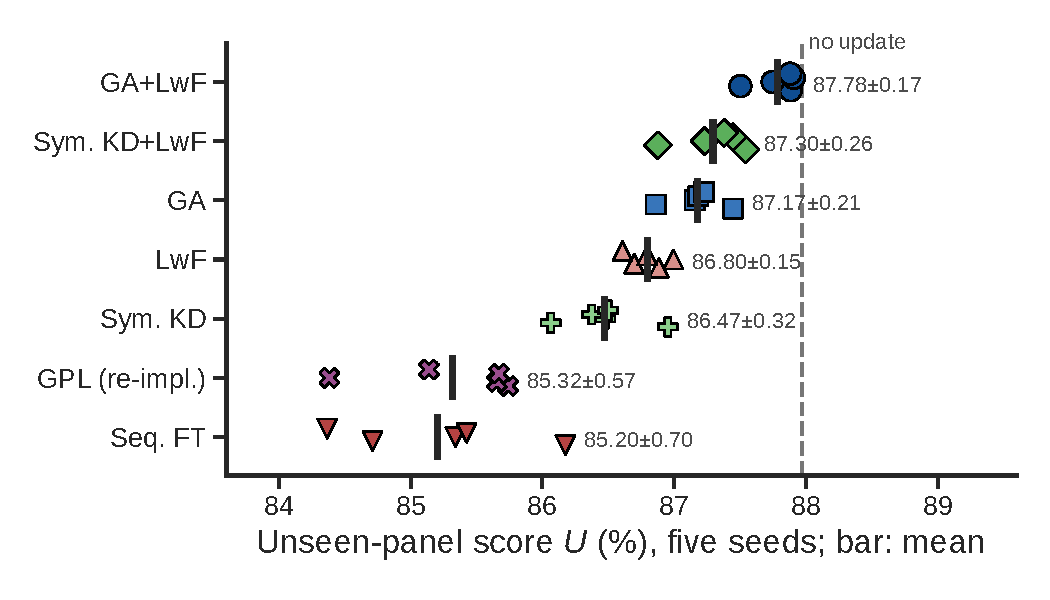
\includegraphics[width=\columnwidth]{figures/fig_seeds.pdf}
\caption{Unseen-panel score of the final S1 models for five training seeds (dots) and their mean (bar). The dashed line is the never-updated detector.}
\label{fig:seeds}
\end{figure}

\textit{Training seeds.}\label{sec:seeds} Table~\ref{tab:seeds} and Fig.~\ref{fig:seeds} repeat the main comparison of stream S1 with five training seeds. A seed changes the few-shot sample of every task and all training randomness; the initial GenD model is the same. The comparisons of the single-seed study hold in every seed. GA+LwF exceeds LwF by 0.99$\pm$0.22 points, sequential fine-tuning by 2.58$\pm$0.65, symmetric KD+LwF by 0.49$\pm$0.10 and GPL by 2.47$\pm$0.60, and GA exceeds symmetric KD by 0.70$\pm$0.13. Each difference is positive in all five seeds, its per-seed bootstrap interval excludes zero in all five seeds, and all five registered tests hold after Holm correction (adjusted $p\le0.0008$). GA+LwF is also among the most stable methods, with a standard deviation of 0.17 points in $U$ (LwF 0.15) against 0.70 for sequential fine-tuning and 0.57 for GPL. Seed 0, used in the single-seed study, was favorable to sequential fine-tuning: its mean over seeds is 85.20, against 86.17 for seed 0, so the single-seed comparisons were conservative. The mean gain of GA+LwF is 47\% of that of sequential fine-tuning (1.31 against 2.81), slightly below the guardrail of one half that held in the confirmation run; the gain of sequential fine-tuning itself varies strongly across seeds (standard deviation 1.46). Averaged over seeds, GA+LwF stays within 0.19 points of the never-updated detector in $U$, while GA alone attains the highest AA (95.29).

\begin{table}[t]
\caption{Five training seeds on stream S1 (mean and standard deviation; test splits with 8 frames per video). The never-updated detector does not depend on the seed.}
\label{tab:seeds}
\centering
\footnotesize
\setlength{\tabcolsep}{2.5pt}
\begin{tabular}{@{}lccccc@{}}
\toprule
Method & $U$ & T2I & AA & Gain & ACC$_{\mathrm{FF}}$ \\
\midrule
No update & 87.97 & 78.02 & 93.27 & \textendash & 94.1 \\
Seq.\ FT & 85.20{\tiny$\,\pm$0.70} & 63.19{\tiny$\,\pm$1.62} & 94.84{\tiny$\,\pm$0.26} & 2.81{\tiny$\,\pm$1.46} & 83.1{\tiny$\,\pm$1.3} \\
LwF & 86.80{\tiny$\,\pm$0.15} & 69.10{\tiny$\,\pm$0.42} & 94.79{\tiny$\,\pm$0.11} & 1.54{\tiny$\,\pm$0.44} & 90.1{\tiny$\,\pm$0.5} \\
Symmetric KD & 86.47{\tiny$\,\pm$0.32} & 67.15{\tiny$\,\pm$0.99} & 94.85{\tiny$\,\pm$0.08} & 1.85{\tiny$\,\pm$0.86} & 88.7{\tiny$\,\pm$1.0} \\
Sym.\ KD+LwF & 87.30{\tiny$\,\pm$0.26} & 71.76{\tiny$\,\pm$0.99} & 94.57{\tiny$\,\pm$0.12} & 1.19{\tiny$\,\pm$0.38} & 92.0{\tiny$\,\pm$0.6} \\
GPL$^\dagger$ & 85.32{\tiny$\,\pm$0.57} & 71.20{\tiny$\,\pm$2.01} & 94.25{\tiny$\,\pm$0.48} & 3.69{\tiny$\,\pm$0.90} & 82.3{\tiny$\,\pm$2.9} \\
GA & 87.17{\tiny$\,\pm$0.21} & 68.96{\tiny$\,\pm$0.77} & 95.29{\tiny$\,\pm$0.14} & 1.95{\tiny$\,\pm$0.88} & 90.4{\tiny$\,\pm$1.2} \\
GA+LwF & 87.78{\tiny$\,\pm$0.17} & 73.36{\tiny$\,\pm$0.90} & 94.84{\tiny$\,\pm$0.15} & 1.31{\tiny$\,\pm$0.41} & 93.2{\tiny$\,\pm$0.7} \\
\bottomrule
\end{tabular}
\end{table}

\textit{Matched plasticity.}\label{sec:matched} Equal weights do not impose equally strong constraints on different losses, so a stronger LwF or a gentler fine-tuning might reach the same trade-off as GA+LwF. We therefore selected, on development data, the setting of each competitor whose mean gain was closest to that of GA+LwF (1.03), from grids registered in advance: LwF with $\lambda_l\in\{1,2,4,10\}$, sequential fine-tuning with learning rate $\{10^{-4},3{\cdot}10^{-5},10^{-5}\}$ and GA alone with $\lambda\in\{1,3,10\}$. The rule chose $\lambda_l=2$, a learning rate of $3{\cdot}10^{-5}$ and $\lambda=3$, and each chosen setting was trained with five seeds (Table~\ref{tab:matched}). On the test data the matched settings learn about as much as GA+LwF (gains 1.07 to 1.61 against 1.31). GA+LwF still retains more than the stronger LwF, by 0.52$\pm$0.06 points of $U$ (positive in all five seeds, Holm-adjusted $p=0.0001$), and the stronger LwF also learns less and reaches a lower AA. GA+LwF retains 0.81$\pm$0.32 points more than the gentler fine-tuning (positive in all five seeds, $p=0.0023$), which learns slightly more. Reducing the learning rate closes most of the gap of plain fine-tuning in $U$, from 2.58 to 0.81 points, but not all of it, and it leaves the fixed-threshold accuracy of the base task at 89.2\% against 93.2\%. Alignment alone at $\lambda=3$ does better than the pre-set combination: it retains 0.17$\pm$0.09 points more $U$ (higher in all five seeds, two-sided $p=0.017$, a descriptive comparison), learns more (gain 1.61) and reaches a higher AA (95.15). Its unseen score, 87.95, equals that of the never-updated detector. On S1 with the CLIP backbone, development-selected GA alone therefore matched or exceeded the default GA+LwF configuration. We did not test this configuration on the other task orders, the PE backbone or the nine-update stream, where all results refer to GA+LwF.

\begin{table}[t]
\caption{Comparison at matched plasticity on stream S1 (five seeds; test splits with 8 frames per video). Matched settings were chosen on development data as those whose development gain is closest to that of GA+LwF; the other rows are the default settings for reference.}
\label{tab:matched}
\centering
\footnotesize
\setlength{\tabcolsep}{1.7pt}
\begin{tabular}{@{}lcccccc@{}}
\toprule
& Dev. & Test & & & & \\
Setting & gain & gain & $U$ & T2I & AA & ACC$_{\mathrm{FF}}$ \\
\midrule
GA+LwF ($\lambda_g=\lambda_l=1$) & 1.03 & 1.31 & 87.78{\tiny$\,\pm$0.17} & 73.36 & 94.84 & 93.2 \\
LwF, $\lambda_l=1$ & 1.29 & 1.54 & 86.80{\tiny$\,\pm$0.15} & 69.10 & 94.79 & 90.1 \\
LwF, $\lambda_l=2$ (matched) & 0.94 & 1.07 & 87.27{\tiny$\,\pm$0.16} & 71.86 & 94.54 & 92.6 \\
Seq.\ FT, lr $10^{-4}$ & 1.58 & 2.81 & 85.20{\tiny$\,\pm$0.70} & 63.19 & 94.84 & 83.1 \\
Seq.\ FT, lr $3{\cdot}10^{-5}$ (matched) & 1.09 & 1.48 & 86.97{\tiny$\,\pm$0.38} & 70.84 & 94.25 & 89.2 \\
GA, $\lambda=1$ & 1.32 & 1.95 & 87.17{\tiny$\,\pm$0.21} & 68.96 & 95.29 & 90.4 \\
GA, $\lambda=3$ (matched) & 1.09 & 1.61 & 87.95{\tiny$\,\pm$0.18} & 73.48 & 95.15 & 93.2 \\
\bottomrule
\end{tabular}
\end{table}

\textit{Nine updates.}\label{sec:long} Representation drift can accumulate over many updates, so we extended stream S1 to nine updates by splitting the fitting pools into disjoint few-shot sessions of 25 genuine and 25 manipulated videos: four sessions of DFDC-P, four of DFD and the single session that the Celeb-DF pool allows. Table~\ref{tab:long} reports the final models. The advantage of GA+LwF grows with the length of the stream. It exceeds LwF by 2.13 ($[+1.46,+2.85]$), GPL by 3.48 ($[+2.09,+4.97]$) and sequential fine-tuning by 5.32 ($[+3.98,+6.77]$), between 1.6 and 3.1 times the margins after three updates, and all three registered hypotheses hold. After nine updates sequential fine-tuning has lost 6.22 points of $U$, its text-to-image AUROC has fallen from 78.02 to 56.46, and its fixed-threshold \ffpp{} accuracy is 68.8\%. GA+LwF loses 0.90 points of $U$, keeps 87.5\% accuracy on \ffpp{}, and also attains the highest AA of all methods (95.17), because it forgets the base task least. Symmetric KD+LwF (85.85) falls further behind GA+LwF than after three updates, which is consistent with the cost of constraining manipulated features accumulating over updates. GPL again learns the new data most (gain 2.25) and forgets the base task most among the regularized methods.

\begin{table}[t]
\caption{Nine-update stream (\ffpp{}, four DFDC-P sessions, four DFD sessions, Celeb-DF), seed 0, after the last update; test AUROC per dataset with 8 frames per video (FF: \ffpp{}).}
\label{tab:long}
\centering
\footnotesize
\setlength{\tabcolsep}{1.1pt}
\begin{tabular}{@{}lccccccccc@{}}
\toprule
Method & $U$ & T2I & FF & DFDC-P & DFD & CDF & AA & Gain & ACC$_{\mathrm{FF}}$ \\
\midrule
No update & 87.97 & 78.02 & 98.06 & 85.71 & 97.38 & 91.92 & 93.27 & \textendash & 94.1 \\
Seq.\ FT & 81.75 & 56.46 & 91.58 & 90.38 & 97.35 & 92.99 & 93.08 & 1.49 & 68.8 \\
LwF & 84.95 & 63.44 & 95.91 & 90.02 & 98.72 & 93.58 & 94.56 & 1.10 & 80.8 \\
Sym.\ KD+LwF & 85.85 & 66.61 & 97.35 & 89.13 & 98.75 & 94.29 & 94.88 & 0.83 & 85.7 \\
GPL$^\dagger$ & 83.59 & 66.67 & 91.82 & 91.97 & 96.11 & 91.25 & 92.79 & 2.25 & 71.8 \\
GA & 85.66 & 63.89 & 96.32 & 89.52 & 99.34 & 95.06 & 95.06 & 1.00 & 81.9 \\
GA+LwF & 87.07 & 70.64 & 97.59 & 89.06 & 99.44 & 94.59 & 95.17 & 0.82 & 87.5 \\
\bottomrule
\end{tabular}
\end{table}

Fig.~\ref{fig:long} follows $U$ after every update, scored with WildDeepfake subsampled to eight frames per sequence. GA+LwF has the highest $U$ after every one of the nine updates and declines slowly, from 87.85 after the first update to 86.91 after the last. Sequential fine-tuning fluctuates strongly from one update to the next, between 81.49 and 86.70, and GPL declines steadily to 83.58. The fourth DFDC-P session lowers $U$ for every method, which again shows that particular data, rather than the number of updates alone, drives the loss of generalization.

\begin{figure}[t]
\centering
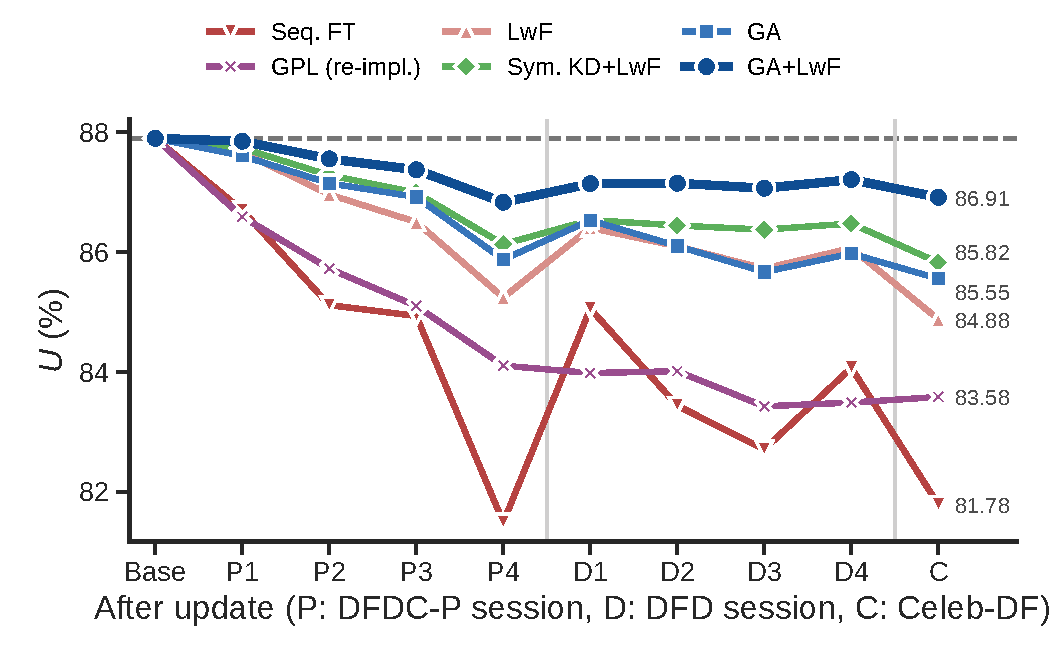
\includegraphics[width=\columnwidth]{figures/fig_long.pdf}
\caption{Unseen-panel score after every update of the nine-update stream (WildDeepfake with eight frames per sequence). The dashed line is the never-updated detector.}
\label{fig:long}
\end{figure}


\begin{figure}[t]
\centering
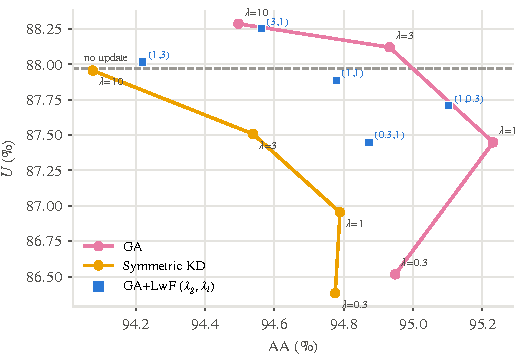
\includegraphics[width=\columnwidth]{figures/fig_lambda.pdf}
\caption{Sensitivity to the distillation weight on stream S1. Each line traces one family over $\lambda\in\{0.3,1,3,10\}$; squares show GA+LwF with weights $(\lambda_g,\lambda_l)$. The genuine-anchored frontier dominates the symmetric one at every weight.}
\label{fig:lambda}
\end{figure}

\textit{Weight sensitivity.}\label{sec:lambda} The weights $\lambda_g=\lambda_l=1$ were fixed in advance. Fig.~\ref{fig:lambda} varies them on stream S1. For every value of $\lambda\in\{0.3,1,3,10\}$, GA attains both a higher $U$ and a higher AA than symmetric KD with the same weight, so the genuine-anchored frontier dominates the symmetric one. A stronger GA weight trades plasticity for retention: at $\lambda=3$ GA reaches $U=88.12$ with AA 94.93, and at $\lambda=10$ it reaches 88.29 with AA 94.50. The pre-set weight is therefore conservative rather than optimal. GA alone at $\lambda=3$ improves on GA+LwF at $\lambda_g=\lambda_l=1$ in $U$, AA and gain, and GA+LwF with $\lambda_g=3$ reaches 88.25. We did not change the reported configuration on the basis of these results, which were obtained on the sealed data. Section~\ref{sec:matched} confirms the observation over five seeds with the weight selected on development data.

\begin{figure}[t]
\centering
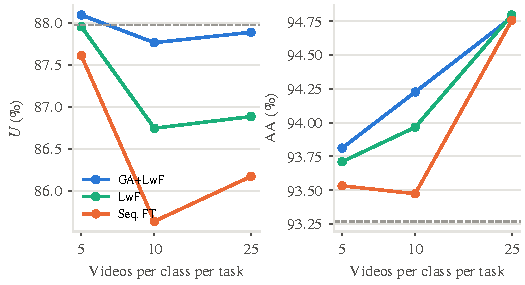
\includegraphics[width=\columnwidth]{figures/fig_shots.pdf}
\caption{Unseen-panel score (left) and mean test AUROC on the trained datasets (right) as a function of the number of videos per class and task. Dashed lines mark the never-updated detector.}
\label{fig:shots}
\end{figure}

\textit{Data regime.} Fig.~\ref{fig:shots} varies the number of videos per class and task. With five videos, no method learns much (gains between 0.11 and 0.22 points), and all methods stay close to the never-updated detector. The ordering is nevertheless preserved, with GA+LwF at 88.09. With ten videos, sequential fine-tuning learns aggressively (gain 1.67) and loses the most generalization ($U=85.64$). GA+LwF retains 87.76 while also reaching the highest AA (94.23), giving the largest advantage in the study: 2.12 points over sequential fine-tuning and 1.01 over LwF. At 25 videos the three methods reach the same AA, and GA+LwF still retains the most generalization.

\begin{figure}[t]
\centering
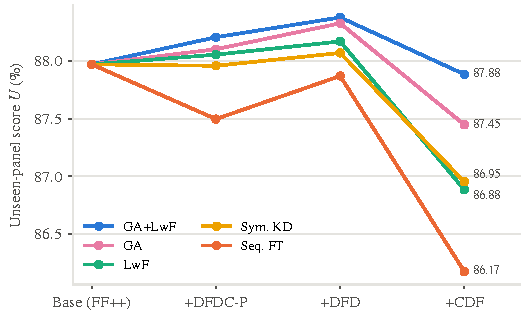
\includegraphics[width=\columnwidth]{figures/fig_stagewise.pdf}
\caption{Unseen-panel score of intermediate models along stream S1. Most of the generalization is lost at the final Celeb-DF update.}
\label{fig:stagewise}
\end{figure}

\subsection{Mechanism and robustness analyses}
\textit{Loss along the stream.} Evaluating the intermediate models on the unseen panel (Fig.~\ref{fig:stagewise}) shows that the loss is not spread evenly over the stream. The first two updates leave the unseen score unchanged or slightly higher for every method except sequential fine-tuning after DFDC-P. Most of the loss occurs at the final Celeb-DF update, where sequential fine-tuning drops from 87.87 to 86.17 and GA+LwF from 88.38 to 87.88. This agrees with the order replication: when CDF is learned before DFD (order S2), all methods lose less. The datasets that most damage generalization are thus specific, and the protection offered by GA matters most at those updates.

\begin{figure}[t]
\centering
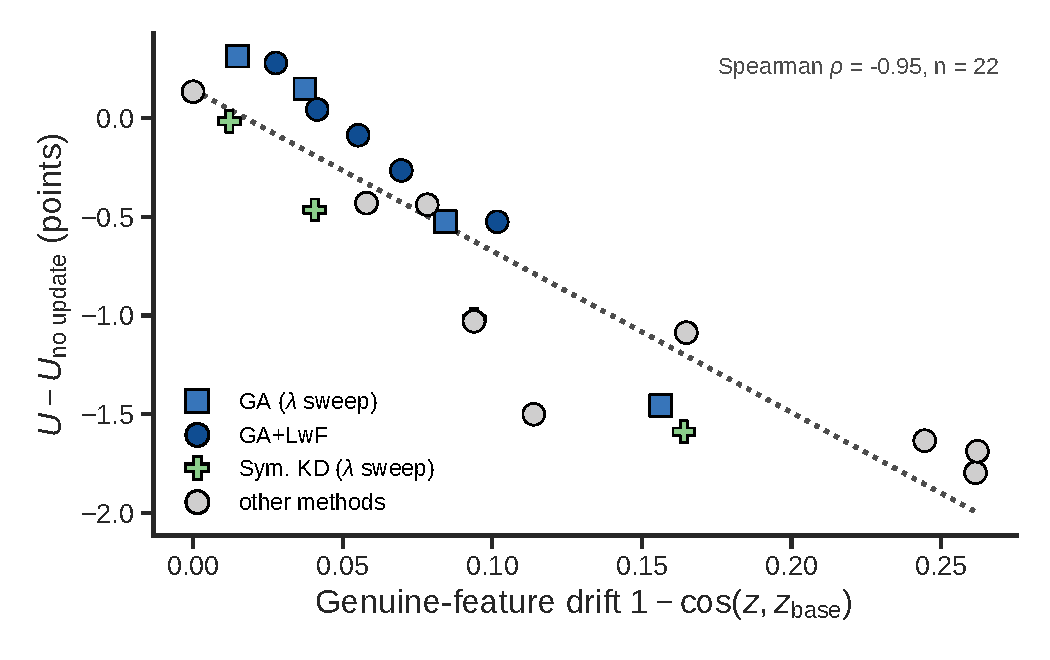
\includegraphics[width=\columnwidth]{figures/fig_drift.pdf}
\caption{Genuine-feature drift of the final model with respect to the initial model versus the change in unseen-panel score, for 22 runs on stream S1 (all methods and weight sweeps).}
\label{fig:drift}
\end{figure}

\textit{Representation drift.}\label{sec:drift} For a fixed probe set of genuine faces, stream manipulations and unseen manipulations, we measured the mean angular drift $1-\cos(z,z_{\mathrm{base}})$ of every final model with respect to the initial model. Across 22 runs, genuine-feature drift predicts the change in $U$ closely (Fig.~\ref{fig:drift}, Spearman $\rho=-0.95$), but drift of manipulated features predicts it equally well ($\rho$ between $-0.93$ and $-0.96$), and the partial correlation of genuine drift given manipulated-feature drift is only $-0.22$. Drift therefore shows that overall representation stability predicts retention, not a genuine-specific mechanism; the matched controls address the latter. GA does change the composition of the drift as intended: its ratio of genuine to stream-manipulation drift is 0.68, against 0.75 for symmetric, random-subset and fake-only KD (0.69 for GA+LwF against 0.79 for symmetric KD+LwF).

The constraint also transfers beyond the data it is applied to, as Section~\ref{sec:theory} requires: GA, trained on genuine faces of the stream datasets only, reduces the drift of genuine faces from WildDeepfake (0.088 against 0.098 for symmetric and random-subset KD and 0.121 for fake-only KD) and from DeepFakeFace (0.060 against 0.064, 0.065 and 0.076), neither of which any model saw.

\begin{figure}[t]
\centering
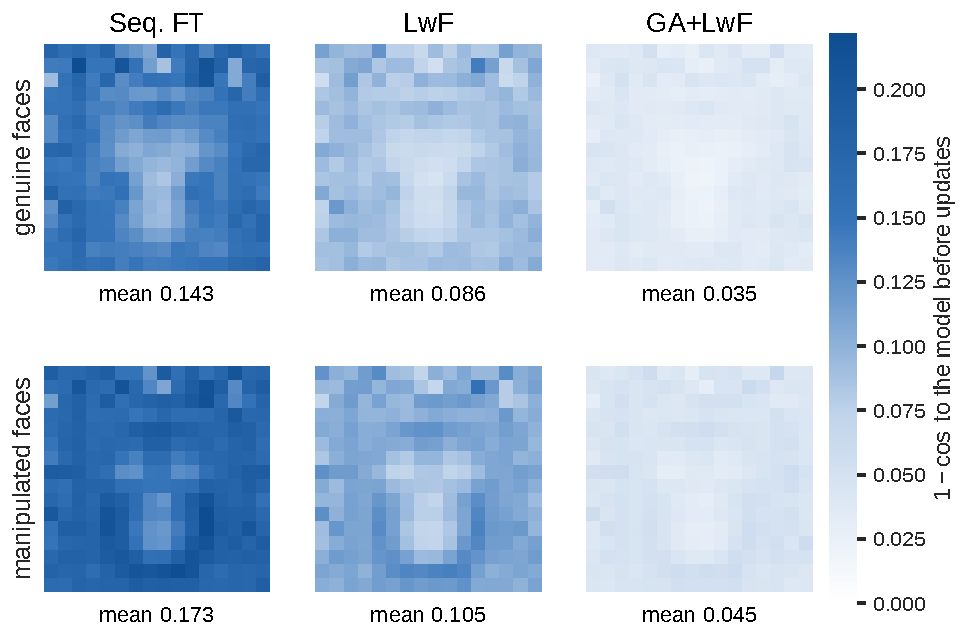
\includegraphics[width=\columnwidth]{figures/fig_driftmaps.pdf}
\caption{Mean drift of last-layer patch tokens with respect to the model before updates, over the probe set of genuine faces (top) and manipulated faces (bottom). Lighter is more stable.}
\label{fig:driftmaps}
\end{figure}

\begin{figure*}[t]
\centering
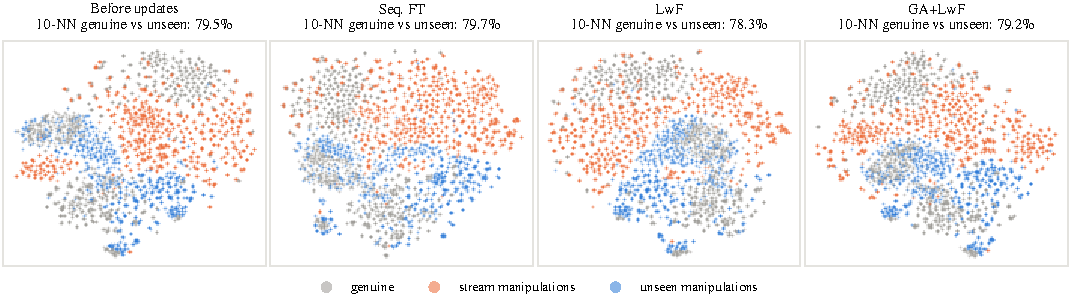
\includegraphics[width=\textwidth]{figures/fig_tsne.pdf}
\caption{t-SNE of probe-set features before updates and after the S1 stream. Titles give the 5-fold accuracy of a 10-nearest-neighbor classifier separating genuine faces from unseen manipulations in the original feature space.}
\label{fig:tsne}
\end{figure*}

On the grid of last-layer patch tokens (Fig.~\ref{fig:driftmaps}), sequential fine-tuning changes every patch, most strongly at the border and in the background; GA+LwF reduces this drift by a factor of four, almost uniformly. A 10-nearest-neighbor classifier separates genuine faces from unseen manipulations with almost the same accuracy for every model (78.3\% to 79.7\%; Fig.~\ref{fig:tsne}), so the information needed to detect unseen manipulations survives every update in the local structure of the representation. What updates damage is its alignment with the linear decision function, consistent with Proposition~\ref{prop:auc}.

\textit{Misranked pairs.} Under its assumptions, Proposition~\ref{prop:auc} implies that an update can only misrank pairs whose margin before the update is small. In a post hoc check on the unseen panel, we took every genuine and manipulated pair that the never-updated model ranks correctly and measured how often the final model misranks it, as a function of the margin $s(u)-s(r)$ in logits before the update (Fig.~\ref{fig:margin}). Misranked pairs are confined to small margins for every method, and no pair with a margin above 8 is lost. GA+LwF loses the fewest pairs in every margin bin among the methods that learn: 3.2\% overall, against 6.4\% for LwF and 8.9\% for sequential fine-tuning.

\begin{figure}[t]
\centering
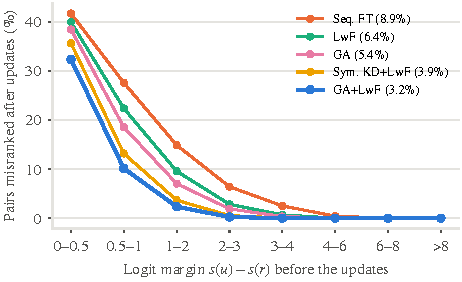
\includegraphics[width=\columnwidth]{figures/fig_margin.pdf}
\caption{Fraction of correctly ranked genuine and manipulated pairs of the unseen panel that are misranked after the S1 updates, by logit margin before the updates (post hoc). Legend: overall fraction.}
\label{fig:margin}
\end{figure}

In individual examples, text-to-image faces flagged with high confidence by the original detector are lost entirely by sequential fine-tuning (for example 0.97 to 0.05) but keep a substantially higher score under GA+LwF (0.24 to 0.70), and the unseen forgeries that GA+LwF misses are ones the original detector itself flagged with low confidence (0.58 to 0.81), consistent with Proposition~\ref{prop:auc}. Gradient saliency maps were not informative.

\textit{Image degradations.}\label{sec:robust} Deployed detectors receive compressed, resized and noisy images. We re-scored the final models on the unseen panel under 13 degradations of the face crops: JPEG compression at quality 75, 50 and 30, Gaussian blur with $\sigma$ of 1, 2 and 3 pixels, Gaussian noise with $\sigma$ of 5, 10 and 20 grey levels, down-scaling by 0.5, 0.35 and 0.25 followed by up-scaling, and down-scaling by 0.5 followed by JPEG at quality 50. WildDeepfake was scored with eight frames per sequence, which changes clean $U$ by at most 0.08 points. Three hypotheses on the mean $U$ over the 13 conditions, $U_{\mathrm{deg}}$, were registered before scoring.

\begin{figure*}[t]
\centering
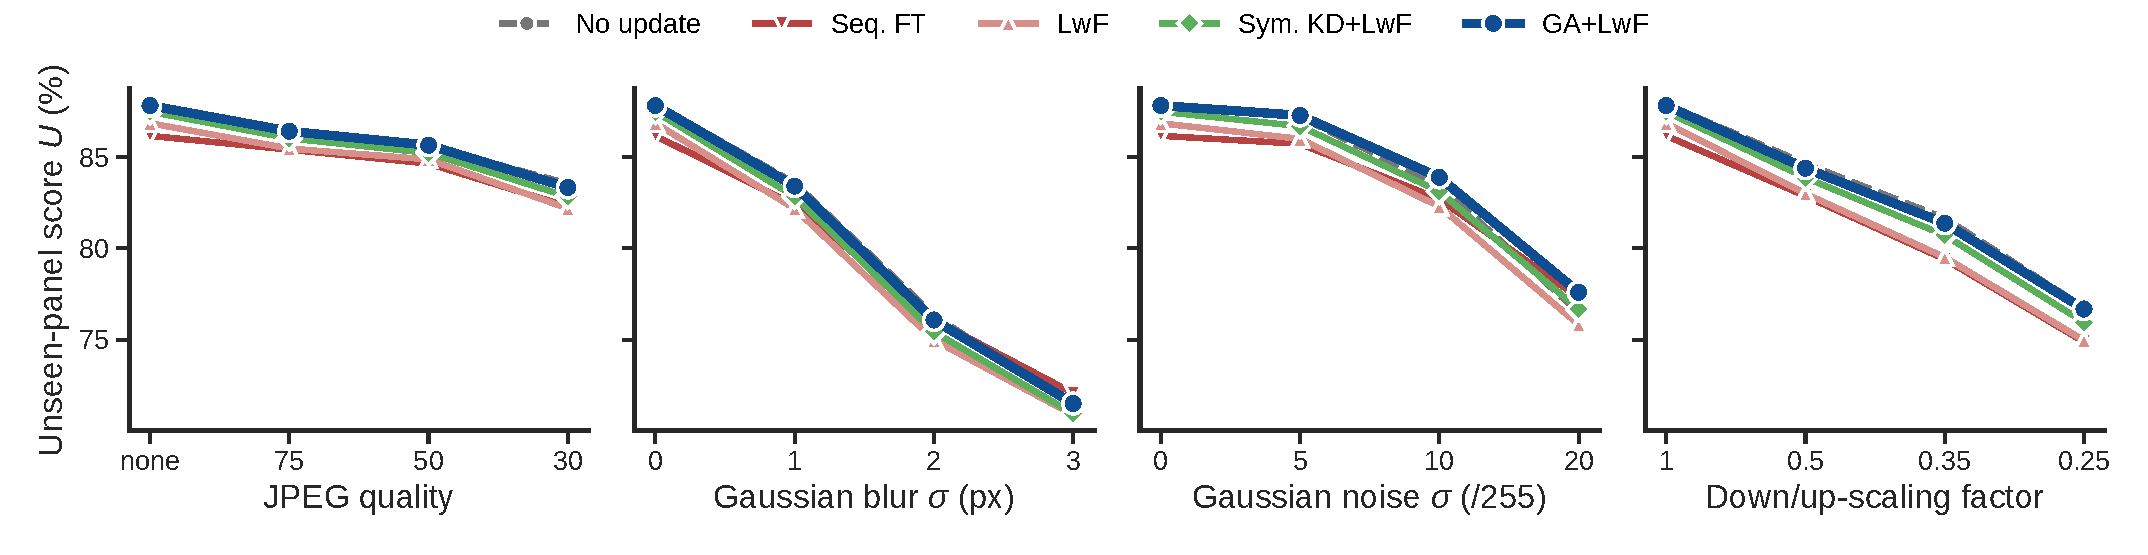
\includegraphics[width=\textwidth]{figures/fig_robust.pdf}
\caption{Unseen-panel score of the final S1 models under JPEG compression, Gaussian blur, Gaussian noise and down/up-scaling of increasing severity (WildDeepfake with eight frames per sequence). The dashed line is the never-updated detector.}
\label{fig:robust}
\end{figure*}

Degradations lower $U$ by 5.6 to 6.5 points on average for every model (Fig.~\ref{fig:robust}). GA+LwF attains the highest $U_{\mathrm{deg}}$ of all nine models, 81.61, equal to that of the never-updated detector (81.55), and all three hypotheses hold: GA+LwF exceeds LwF by 1.27 points ($[+0.94,+1.66]$) and sequential fine-tuning by 0.98 ($[+0.33,+1.66]$), and GA exceeds symmetric KD by 0.73 ($[+0.50,+1.00]$). GA+LwF is the best updated model in 10 of the 13 conditions; under strong blur and noise the differences shrink to a few tenths of a point, and sequential fine-tuning and EWC even exceed the never-updated detector at the strongest blur, presumably because the stream contains low-quality video. Down-scaling separates the methods most clearly: at a factor of 0.35, sequential fine-tuning loses 2.25 points relative to the never-updated detector and GA+LwF 0.28.

\begin{table}[t]
\caption{32-frame evaluation and calibration of final models on stream S1. AA$_{32}$: mean test AUROC with 32 frames; ECE: expected calibration error (15 bins) on test splits and on the unseen panel; FPR: mean false-positive rate on genuine test videos at threshold 0.5.}
\label{tab:calib}
\centering
\footnotesize
\setlength{\tabcolsep}{3.5pt}
\begin{tabular}{@{}lcccc@{}}
\toprule
Method & AA$_{32}$ & ECE (test) & ECE (panel) & FPR (\%) \\
\midrule
No update & 93.33 & 0.056 & 0.061 & 22.1 \\
Head-only FT & 93.35 & 0.063 & 0.056 & 16.9 \\
Seq.\ FT & 95.06 & 0.040 & 0.118 & 4.3 \\
EWC & 95.06 & 0.041 & 0.113 & 3.7 \\
Replay & 95.06 & 0.040 & 0.124 & 3.5 \\
LwF & 94.97 & 0.056 & 0.090 & 5.5 \\
Symmetric KD & 95.04 & 0.044 & 0.100 & 5.3 \\
Symmetric KD + LwF & 94.71 & 0.066 & 0.081 & 8.6 \\
GA & 95.44 & 0.050 & 0.113 & 6.3 \\
GA+LwF & 94.85 & 0.072 & 0.081 & 9.7 \\
\bottomrule
\end{tabular}
\end{table}

\subsection{Ranking, decisions, calibration and cost}
\label{sec:calib}
AUROC measures how well a model ranks manipulated above genuine videos; deployment also depends on the decisions taken at a threshold and on whether confidence matches correctness. Rescoring the final models with all 32 frames per video changes AA by at most 0.3 points and preserves the ordering of Table~\ref{tab:main}. The never-updated model reproduces the scores of the original training run exactly (98.21 on \ffpp{} and 92.04 on Celeb-DF). Table~\ref{tab:calib} reports calibration. On the unseen panel, GA+LwF is better calibrated than sequential fine-tuning (ECE 0.081 against 0.118). On the test splits of the trained datasets, however, its calibration is worse (0.072 against 0.040), and its false-positive rate on genuine videos at threshold 0.5 is 9.7\% against 4.3\%. This is consistent with its lower plasticity: the trained datasets are learned less completely, so their operating point shifts less. Its accuracy at the fixed threshold is nevertheless the highest among the updated models (87.6\% averaged over the four test splits, against 83.3\% for sequential fine-tuning and 85.0\% for LwF), because the base task keeps its operating point.

Thresholds of 0.5 are rarely used in deployment, where an operator fixes an acceptable false-positive rate instead. For each final model we therefore set the threshold at which 5\% of the pooled genuine development videos of the four trained datasets are flagged, and applied it to the test splits and to the unseen panel (Table~\ref{tab:oppoint}, 32 frames per video). On the test splits the realized false-positive rate stays close to its target (5.6\% to 7.5\%), and GA+LwF detects 81.9\% of the manipulated videos, against 83.0\% for sequential fine-tuning, 81.7\% for LwF and 86.0\% for GA alone. On the unseen panel the threshold does not transfer: every model flags between 22.5\% and 29.5\% of the genuine WildDeepfake videos (21.7\% for EWC and replay, which are not shown), and the false-positive rates on DeepFakeFace genuine images also differ between models (3.3\% to 7.4\%). At these unequal false-positive rates the detection rates of unseen forgeries do not favor GA+LwF: its threshold is the strictest on DeepFakeFace genuine images (3.3\%), and it detects the fewest unseen forgeries (58.0\% on average, against 59.9\% for sequential fine-tuning). When the threshold is instead set on each unseen dataset itself at 5\% false positives, which isolates the ranking in the low false-positive region, GA+LwF detects 57.7\% of the unseen forgeries on average over five seeds, as many as the never-updated detector (57.6\%), against 53.9\% for sequential fine-tuning, 55.6\% for LwF and 47.9\% for GPL; this comparison was added after the registration. Neither diagnostic is a deployable threshold-selection procedure under the exemplar-free constraint: the first pools genuine development videos of all earlier tasks, which an exemplar-free update does not retain, and the second uses labelled data of the evaluation domain itself, so its detection rates describe the ROC curve rather than performance achievable without target-domain calibration. The ranking advantage therefore extends to the low false-positive region of the ROC curve, but no update rule we tested keeps a threshold selected on historical data valid on new domains.

\begin{table}[t]
\caption{Low false-positive operating points of the final S1 models (32 frames per video for test splits). Dev.\ threshold: flags 5\% of the pooled genuine development videos of all trained datasets (requires historical data; seed 0); test and panel TPR/FPR at that threshold, panel TPR averaged over the four unseen sets. Per-set threshold: TPR at 5\% FPR on each unseen set (requires labelled target-domain data), mean over sets and over five seeds, and for text-to-image faces (T2I).}
\label{tab:oppoint}
\centering
\footnotesize
\setlength{\tabcolsep}{2.0pt}
\begin{tabular}{@{}lccccccc@{}}
\toprule
& \multicolumn{5}{c}{Dev.\ threshold} & \multicolumn{2}{c}{Per-set threshold} \\
\cmidrule(lr){2-6}\cmidrule(lr){7-8}
& \multicolumn{2}{c}{Test} & Panel & \multicolumn{2}{c}{Panel FPR} & Panel & \\
Method & TPR & FPR & TPR & WDF & DFF & TPR & T2I \\
\midrule
No update & 78.2 & 6.4 & 61.3 & 27.3 & 4.3 & 57.6 & 37.6 \\
Seq.\ FT & 83.0 & 7.3 & 59.9 & 22.5 & 4.8 & 53.9 & 21.8 \\
LwF & 81.7 & 5.7 & 58.8 & 22.5 & 4.2 & 55.6 & 26.4 \\
Sym.\ KD+LwF & 82.1 & 7.3 & 60.1 & 26.3 & 4.0 & 57.1 & 30.2 \\
GPL$^\dagger$ & 82.3 & 5.6 & 61.9 & 29.5 & 7.4 & 47.9 & 23.6 \\
GA & 86.0 & 7.4 & 59.5 & 26.3 & 3.7 & 57.2 & 27.6 \\
GA+LwF & 81.9 & 6.6 & 58.0 & 22.7 & 3.3 & 57.7 & 31.2 \\
\bottomrule
\end{tabular}
\end{table}

An obvious remedy is to recalibrate after each update with the only data available, those of the current task. A bias or a Platt scaling map fitted on 25 genuine and 25 manipulated Celeb-DF development videos reduces the test ECE of GA+LwF from 0.072 to 0.054 with Platt scaling, but the same map roughly doubles the ECE on the unseen panel for every model (for GA+LwF from 0.081 to 0.167), because the slope learned on the newest task, above 2 for every updated model, sharpens all scores. Recalibration on the newest data alone therefore does not transfer, and calibration after an update needs either a calibration set covering several sources or an update rule that preserves it.


\textit{Computational cost.} GA and GA+LwF add one forward pass of the frozen previous model per batch: the three-task stream takes 14.9 minutes against 10.7 for sequential fine-tuning, as for LwF and symmetric KD, and peak memory rises from 5.42 to 5.50~GiB. Nothing is stored between updates and inference is unchanged, whereas replay must store raw face videos of real people.

\section{Discussion}
\label{sec:discussion}

\subsection{Interpretation}
The results support a consistent picture. For a parameter-efficient foundation detector, the representation of manipulated faces must change to accommodate a new forgery, but the representation of genuine faces need not. Unseen manipulations are implicitly compared against that genuine representation. Aligning only genuine faces, as DFWF proposed for spoofed speech, preserves it at a smaller cost in plasticity than aligning all faces. The matched controls show that the benefit is tied to the genuine class rather than to a weaker constraint, the weight sweep shows that it holds at every strength, and the comparison at matched plasticity shows that neither a stronger LwF nor a gentler fine-tuning reaches the same retention, while on S1 with the CLIP backbone alignment alone with a development-selected weight does slightly better than the combination. Logit distillation stabilizes the output distribution and was complementary at the pre-set weights. That an objective designed for audio transfers to visual face forgery detection, and outperforms a recent specialized visual method, suggests that the asymmetry between one shared genuine class and many manipulated classes is a property of forgery detection rather than of a modality.

\subsection{Practical guidance}
Three observations translate into recommendations. First, retention of generalization should be measured at every update, because forgetting metrics on the trained datasets barely register the damage. Second, genuine-sample alignment is a useful baseline for exemplar-free updates of LayerNorm-tuned foundation detectors in the tested setting, not a guarantee of retention: text-to-image faces still lose performance and decision thresholds do not transfer. Its weight should be chosen on development data according to how much plasticity the application needs; on S1 with the CLIP backbone, alignment alone with a weight chosen this way matched or exceeded the combination with LwF in retention, learning and AA, so the LwF term may be unnecessary, although we did not verify this in the other settings. Third, calibration should be monitored after every update. Fitting a recalibration map on the newest data alone improved calibration on the trained datasets but degraded it on unseen data, so a calibration set should cover more than the latest source.

\subsection{Limitations}
Several limitations qualify these conclusions. The update objective is prior work~\cite{ma2021dfwf}; this study adds evidence about it in a new modality and regime. Retention is uneven across forgery families: the aggregate score hides a loss on text-to-image faces that no method avoided. Five seeds were run only for the main comparison on S1, all from the same GenD model, so variability of the base training is not covered, and the development-selected GA-only configuration was tested only on S1. GPL was compared through our re-implementation, with unreported settings fixed in advance. The sealed panel was re-used across extension stages, although no decision was based on it, and the method was refined on development data before confirmation. Manipulated \ffpp{} and DFD videos were cropped with masks; with label-independent crops DFD AUROC is 4.5 to 6.6 points lower for every model, although the comparison between methods changes little (Section~\ref{sec:labelindep}). DeepFakeFace consists of single images, WildDeepfake and DFDC-P are re-aligned from distributed crops, the nine-update stream draws on three datasets, and all detectors are GenD variants. The robustness study uses synthetic degradations, and the margin analysis is post hoc. Finally, GA learns the new datasets less completely than sequential fine-tuning, and its calibration on them is worse.

\section{Conclusion}

We studied how a generalizable foundation-model deepfake detector should be updated when new manipulations appear. For GenD, few-shot updates cause little conventional forgetting but erode generalization to unseen manipulations and the calibration of the original task. Genuine-sample alignment, introduced for continual fake-audio detection, transfers to this visual setting: combined with logit distillation, it keeps generalization on sealed unseen datasets close to that of the never-updated model while still improving the new datasets, without storing data, adding parameters or changing inference. Matched controls tie the effect to the genuine class, and a ranking-margin analysis provides a conditional interpretation. At matched plasticity it retains more than a stronger LwF or a gentler fine-tuning, and on the main stream with the CLIP backbone alignment alone with a development-selected weight matched or exceeded the combination. The result holds over five training seeds, task orders, a second encoder, image degradations and a nine-update stream, where its advantage grows, and against a re-implementation of the specialized GPL method. Retention is incomplete for fully synthetic faces, and calibration and decision thresholds after updates remain open: thresholds selected on development data do not transfer to unseen data for any method we tested. Future work should test streams of genuinely new generators, full-data updates and other parameter-efficient detectors, and develop calibration methods that survive exemplar-free updates.

\balance
\bibliographystyle{IEEEtran}
\bibliography{references}

\end{document}
